\documentclass[sigconf,nonacm]{acmart}
\usepackage{algorithm}
\usepackage{algpseudocode}
\usepackage{booktabs}
\usepackage{amsmath}
\usepackage{url}
\usepackage{hyperref}
\usepackage{dblfloatfix}

\renewcommand{\topfraction}{0.95}
\renewcommand{\bottomfraction}{0.95}
\renewcommand{\textfraction}{0.05}
\renewcommand{\floatpagefraction}{0.85}
\renewcommand{\dbltopfraction}{0.95}
\renewcommand{\dblfloatpagefraction}{0.85}
\setcounter{dbltopnumber}{3}
\setcounter{topnumber}{4}
\setcounter{bottomnumber}{4}
\setcounter{totalnumber}{6}

\begin{document}

\title{MORONI: Polygon-Guided Cellular Textures via Roots-of-Unity Polygons and Phase-Modulated Boundaries}

\author{Phani Srikar}
\affiliation{\institution{Independent Researcher}\city{}\country{}}

\begin{abstract}
Voronoi and Worley noise are foundational cellular primitives in real-time
graphics, but offer limited art direction. Under nearest-site assignment,
every cell boundary is constrained to be a perpendicular bisector, preventing
artists from directly prescribing target polygon silhouettes, uniform grout
widths, or non-linear crack-like seams.

This paper presents \textbf{MORONI}, a controllable cellular texture technique
that parameterizes cells as jittered roots-of-unity polygons and assigns pixels
via a three-term energy combining center distance, signed polygon distance, and
an angular phase-interference field. A signed distance field directs interior
pixel assignment toward polygon medial axes, while an optional coverage margin
$m$ clips assigned regions to release cells from the strict space-filling
constraint. Quantitative ablation demonstrates that clipping recovers target
silhouettes across polygon classes (raising triangular shape IoU from $0.491$ to
$0.876$ for Voronoi and $0.890$ for MORONI), while MORONI's signed energy refines
the boundary partition between competing adjacent cells (+0.0130 IoU for
triangles) and provides a monotonic grout width dial ($51\%$ to $93\%$ coverage).
Furthermore, angular phase interference enables non-convex cell boundaries
($100\%$ at $\gamma \ge 0.20$) and multi-pixel disconnected lobes ($7.3\%$ at
$\gamma = 0.35$ after filtering 1-pixel raster artifacts), departing from the
convex and connected topologies enforced by power and additively weighted
Voronoi diagrams.

For offline CPU synthesis, an admissible incumbent-based lower bound enables
exact candidate cell pruning, which, together with lattice binning and algebraic
elimination of \texttt{atan2}, accelerates evaluation by $4.8\times$ over brute
force with identical pixel labels. Bilinear interpolation of the signed-field
lookup table achieves a mean absolute distance error of $9.2 \times 10^{-5}$ and
a label mismatch rate of $0.030\%$ against analytical polygon distance at
$72\times72$ resolution. For real-time pipelines, we implement a GPU WebGL2
fragment shader evaluating analytical polygon SDFs and phase modulation at 60+
FPS ($<1.0$\,ms at 1080p), accompanied by an open-source companion studio with
live PBR texture generation (diffuse, normal, height, roughness) and vector SVG
export, hosted at \url{https://pikachuxxxx.github.io/Moroni-Studio/} with code
and reproduction suites at \url{https://github.com/Pikachuxxxx/Moroni-Studio}.
\end{abstract}

\keywords{procedural texture, cellular noise, Voronoi diagram, signed distance field,
roots of unity, phase modulation, real-time rendering, WebGL}
\maketitle

\section{Introduction}

Cellular noise is foundational to procedural visual effects, game rendering,
and virtual worlds. Natural and architectural surfaces --- cracked desert mud,
masonry stone walls, ceramic floor tiles, shattered glass, reptilian scales, and
weathered paint --- exhibit characteristic cellular tiling structures. In modern
real-time pipelines (Unreal Engine Material Graph, Unity Shader Graph, Blender
Cycles/EEVEE, and Substance 3D Designer), Voronoi and Worley
noise~\cite{voronoi1908,worley1996} dominate because they require negligible
memory, evaluate rapidly, and possess simple closed-form formulations.

Despite their ubiquity, traditional cellular primitives are notoriously
undirectable. Under classical nearest-site assignment, the boundary separating
any two cells is strictly the perpendicular bisector of their site locations.
Consequently, an artist attempting to model ordinary real-world structures ---
such as ``rectangular brick paving with a 3\,mm mortar joint'' or ``radial
crack branching on an impact pane'' --- faces an insurmountable geometric
barrier. Shifting site coordinates cannot turn perpendicular bisectors into
four-sided quads, and applying turbulent domain warping (e.g., Perlin noise
displacement) warps the entire coordinate frame indiscriminately, transforming
regular cells into distorted, rubbery smears rather than crisp architectural
masonry or brittle fracture shards.

Weighted diagram generalizations relax the perpendicular bisector constraint,
but remain structurally constrained. Power (Laguerre)
diagrams~\cite{aurenhammer1987power} replace Euclidean distance
$\lVert\mathbf{x}-\mathbf{u}_c\rVert$ with $\lVert\mathbf{x}-\mathbf{u}_c\rVert^2 - w_c$,
and additively weighted (Apollonius) diagrams replace it with
$\lVert\mathbf{x}-\mathbf{u}_c\rVert - w_c$. However, power diagram cells are
intersections of affine half-planes and are mathematically guaranteed to be
strictly \emph{convex}; Apollonius cells are guaranteed to be strictly
\emph{connected}. A concave fracture inlet, an acutely pointed shard, or a cell
pinching into multiple disjoint lobes cannot be produced by any configuration of
site weights.

\paragraph{Two Geometric Challenges in Polygon-Guided Cellular Synthesis.}
Bridging the gap between procedural efficiency and art directability requires
attaching explicit target polygons to cells. However, constructing an energy
field over polygon cells introduces two distinct geometric challenges:
\begin{enumerate}
\item \textbf{The Boundary Distance Dilemma}: An unsigned distance
$\operatorname{dist}(\mathbf{x},\partial P_c)$ achieves its minimum \emph{on}
the boundary outline $\partial P_c$. Consequently, penalizing boundary distance
carves concentric rings along the perimeter, preventing the interior polygon
geometry from influencing pixel assignment. The boundary field must be
\emph{signed} (negative inside), placing the energy minimum on the polygon's
medial axis (\S\ref{sec:signed}).
\item \textbf{Space-Filling Constraint vs.\ Target Silhouettes}: Under a strict
space-filling $\arg\min$ partition, every pixel must be assigned to some cell,
leaving no unassigned space. For jittered sites, adjacent cells compete along
their common borders, distorting target shapes (such as triangles or quads)
into irregular polygons with compromise edges. Recovering clean target
silhouettes requires decoupling cell assignment from strict space filling.
Introducing a coverage margin $m$ releases pixels whose distance exceeds a
threshold, allowing cells to preserve their prescribed silhouettes while
simultaneously providing an independent, monotonic grout dial (\S\ref{sec:margin}).
\end{enumerate}

\paragraph{Summary of Contributions.}
\begin{itemize}
\item A controllable cellular texture technique parameterizing cells as
jittered roots-of-unity polygons and assigning pixels via a three-term energy
combining center distance, signed polygon distance, and angular phase
interference (\S\ref{sec:method}).
\item A rigorous ablation isolating the roles of polygon clipping and energy
assignment: polygon clipping releases cells from the space-filling constraint
(raising triangular shape IoU from $0.491 \to 0.876$ for Voronoi and $0.890$
for MORONI), while MORONI's signed energy refines boundary arbitration between
competing adjacent cells (+0.0130 IoU for triangles) and provides a monotonic
grout width dial ($51\% \to 93\%$) (\S\ref{sec:control}).
\item A topological analysis demonstrating that angular phase interference
enables non-convex boundaries ($100\%$ at $\gamma \ge 0.20$) and multi-pixel
disconnected lobes ($7.3\%$ at $\gamma = 0.35$ after filtering 1-pixel grid
noise), departing from the convex and connected topologies enforced by power
and additively weighted Voronoi diagrams (\S\ref{sec:reach}).
\item An admissible incumbent-based lower bound enabling exact candidate cell
pruning, combined with lattice binning and algebraic elimination of
$\operatorname{atan2}$ for integer harmonics, accelerating CPU evaluation by
$4.8\times$ over brute force with identical pixel labels (\S\ref{sec:fast}).
\item Rigorous numerical error analysis of bilinear signed-field lookup table
(LUT) sampling, achieving a distance MAE of $9.2 \times 10^{-5}$ and a label
mismatch of $0.030\%$ against analytical polygon distance at $72\times72$
resolution (\S\ref{sec:lut_eval}).
\item A real-time GPU WebGL2 fragment shader evaluating analytical polygon SDFs
and phase modulation at 60+ FPS ($<1.0$\,ms at 1080p), accompanied by an
open-source companion studio with live PBR texture generation and vector SVG
export (\S\ref{sec:app}).
\item Full generator algorithms and a comparative operational matrix
contrasting existing cellular schemes against MORONI (Appendix~\ref{sec:appendix_generators}).
\end{itemize}

\section{Related Work}
\label{sec:related}

Procedural pattern synthesis in computer graphics spans gradient noise, cellular
diagrams, distance fields, and physical simulation.

\subsection{Procedural Noise Functions}
Procedural noise began with Perlin's gradient noise~\cite{perlin1985}, followed
by multi-scale spectral representations such as wavelet noise by Cook and
DeRose~\cite{cook2005wavelet}. Lagae et al.~\cite{lagae2009gabor} introduced Gabor
noise, enabling exact spectral control via sparse convolution. The comprehensive
survey by Lagae et al.~\cite{lagae2010noise} traces procedural texturing
through modern physically based production systems~\cite{pbr4}. While gradient
and Gabor noise excel at continuous, band-limited phenomena (clouds, marble, wood
grain), they cannot natively synthesize piecewise partitions, cell boundaries,
or sharp fracture cracks.

\subsection{Cellular Diagrams and Weighted Extensions}
Cellular noise descends from Georgy Voronoi's 1908 treatise on quadratic
forms~\cite{voronoi1908}. Steven Fortune~\cite{fortune1987} pioneered optimal
sweepline geometry for planar Voronoi diagrams. Lloyd~\cite{lloyd1982} introduced
iterative centroidal Voronoi relaxation, widely adopted in graphics for stippling
and remeshing. Steven Worley~\cite{worley1996} revolutionized shader texturing by
introducing the cellular basis function $F_k(\mathbf{x})$, measuring distances
to the $k$-th nearest feature points on a spatial grid, later extended and mapped
efficiently to GLSL by McEwan et al.~\cite{mcewan2012noise}.

To provide size control, weighted Voronoi diagrams were introduced. In Power
diagrams (Laguerre geometry)~\cite{aurenhammer1987power}, each site carries a
scalar weight $w_c$ subtracting from squared distance:
$\lVert\mathbf{x}-\mathbf{u}_c\rVert^2 - w_c$. Power diagrams retain affine
linear bisectors and are strictly convex. In additively weighted (Apollonius)
diagrams, weights subtract directly from Euclidean distance:
$\lVert\mathbf{x}-\mathbf{u}_c\rVert - w_c$, producing hyperbolic curved
boundaries. However, as established in \S\ref{sec:reach}, neither weighted family
can synthesize non-convex shards or disconnected fracture lobes.

\subsection{Procedural Fracture vs.\ Physical Simulation}
Physical fracture modeling accurately simulates crack propagation using finite
element methods (FEM) or boundary element methods (BEM). O'Brien and
Hodgins~\cite{obrien1999fracture} established continuum mechanics fracture for
graphics. Desbenoit et al.~\cite{desbenoit2005cracks} modeled surface cracks and
peeling patterns, and Nealen et al.~\cite{nealen2006survey} surveyed physically
based deformable models. While physically realistic, dynamic FEM/BEM
simulations require minutes to hours of compute per frame, rendering them
unusable for runtime fragment shaders.

Procedural crack generation offers a lightweight alternative. Mould~\cite{mould2005fracture}
synthesized image-guided surface crack patterns using shortest-path graph propagation
on lattices. However, graph-based procedural crack methods operate globally over
memory-resident topologies, preventing parallel, memory-free evaluation in
per-pixel GPU shaders. MORONI achieves real-time procedural fracture directly
in fragment shaders via angular phase interference.

\subsection{Implicit Surfaces and Distance Fields}
Distance transforms map discrete masks to continuous distance
fields~\cite{felzenszwalb2004dt}. Hart~\cite{hart1996spheretracing} demonstrated
sphere tracing against implicit signed distance fields (SDF). In real-time
demoscene and shader art, signed distance functions enable compact procedural
modeling. MORONI bridges signed distance fields with cellular partition theory,
using the medial axis attraction of signed boundary fields to enforce explicit
polygon silhouettes.

\subsection{Controllability in Procedural Content Generation}
Controllability is the central challenge in procedural content generation (PCG).
Smelik et al.~\cite{smelik2014survey} and Vanegas et
al.~\cite{vanegas2010modelling} emphasize that procedural algorithms must provide
intuitive, declarative handles rather than opaque mathematical parameters.
M{\"u}ller et al.~\cite{muller2006buildings} demonstrated rule-based grammar
derivation for procedural architecture, showing that uncontrollable procedural
primitives fail in commercial pipelines. MORONI specifically addresses
controllability by exposing five orthogonal, intuitive dials: shape, size,
irregularity, grout width, and fracture intensity.

\section{Method}
\label{sec:method}

\subsection{Cell Parameterization}

Each cell $c \in \{1,\dots,N\}$ owns a center $\mathbf{u}_c$ and an explicit
$n_c$-gon $P_c$ whose vertices are generated as jittered roots of unity:
\begin{equation}
z_{c,k} = r_c\exp\!\Bigl(i\bigl(\tfrac{2\pi k}{n_c}+\delta_{c,k}\bigr)\Bigr),
\quad \delta_{c,k}\sim\mathcal{U}(-J,J),
\label{eq:poly}
\end{equation}
for $k = 0,\dots,n_c-1$, offset by cell center $\mathbf{u}_c$. Centers are
positioned on a jittered Cartesian lattice of spacing $s$:
\begin{equation}
\mathbf{u}_c = \begin{pmatrix} c_x \cdot s + \xi_{c,x} \\ c_y \cdot s + \xi_{c,y} \end{pmatrix},
\quad \xi_{c,x}, \xi_{c,y} \sim \mathcal{U}(-0.13s, 0.13s).
\end{equation}
Here, $n_c$ governs target cell shape (e.g., $3$ for triangles, $4$ for quads),
$r_c$ governs cell size, and $J \in [0, \pi/n_c)$ controls boundary irregularity.

\subsection{Signed Boundary Field}
\label{sec:signed}

Let $P_c$ denote the polygon of Eq.~\ref{eq:poly}. We define the signed boundary
distance field $s_c(\mathbf{x})$:
\begin{equation}
s_c(\mathbf{x}) =
\begin{cases}
-\operatorname{dist}(\mathbf{x},\partial P_c) & \mathbf{x}\in P_c\\
+\operatorname{dist}(\mathbf{x},\partial P_c) & \text{otherwise,}
\end{cases}
\label{eq:sdf}
\end{equation}
where $\operatorname{dist}(\mathbf{x},\partial P_c) = \min_{\mathbf{y}\in\partial P_c} \lVert\mathbf{x}-\mathbf{y}\rVert_2$.

\paragraph{Mathematical Rationale for the Signed Field.}
Consider an energy term based on unsigned distance
$\beta \operatorname{dist}(\mathbf{x}, \partial P_c)$. Because
$\operatorname{dist} \ge 0$ with $\operatorname{dist}(\mathbf{x}, \partial P_c) = 0$
precisely on the perimeter $\partial P_c$, the term attains its minimum along the
boundary. This creates an energy depression around the perimeter, carving hollow
rings while leaving the cell interior dominated by center distance
$\alpha d_c$. Consequently, the polygon's silhouette never pulls the cell interior.
With Eq.~\ref{eq:sdf}, $s_c(\mathbf{x})$ decreases monotonically toward the
medial axis of $P_c$ ($\min s_c = -I_c < 0$), ensuring that increasing $\beta$
attracts pixel assignment toward the polygon silhouette. Figure~\ref{fig:shape}
verifies this phenomenon.

\subsection{The Three-Term Energy Formulation}

Let $\mathbf{d} = \mathbf{x} - \mathbf{u}_c$, $d_c = \lVert\mathbf{d}\rVert_2$,
and $\theta_c = \operatorname{atan2}(d_y, d_x)$. We assign each pixel
$\mathbf{x}$ to the cell minimizing:
\begin{equation}
E_c(\mathbf{x}) = \underbrace{\alpha d_c}_{\text{size}}
+ \underbrace{\beta\,s_c(\mathbf{x})}_{\text{shape}}
+ \underbrace{\gamma\bigl(1-\cos(\kappa\theta_c+\lambda d_c)\bigr)}_{\text{fracture}},
\label{eq:energy}
\end{equation}
\begin{equation}
L(\mathbf{x}) = \arg\min_{c \in \{1,\dots,N\}} E_c(\mathbf{x}).
\label{eq:argmin}
\end{equation}
Default weights are $\alpha=0.58$, $\beta=0.32$, $\gamma=0.10$, $\kappa=2$, and
$\lambda=1$. Setting $\beta = \gamma = 0$ collapses $E_c(\mathbf{x})$ to
$\alpha d_c$, recovering standard Voronoi exactly.

The phase term $\gamma(1 - \cos(\kappa\theta_c + \lambda d_c))$ acts as an
angular standing wave propagating radially outward. Because neighbouring cells
have independent centres, their respective polar angle frames $\theta_i, \theta_j$
interfere chaotically in contested border regions, causing cell boundaries to
deviate from straight bisectors into intricate, wandering crack paths.

\subsection{Coverage Margin and Space-Filling Decoupling}
\label{sec:margin}

Equation~\ref{eq:argmin} assigns every pixel, producing a space-filling partition of
the image domain. Under point-site Voronoi assignment with jittered positions, cell
boundaries are formed by perpendicular bisectors that generically intersect at 3-valent
junctions; as a result, cells cannot conform to prescribed target silhouettes (such as
equilateral triangles or rectangles) without distorting neighboring boundaries. Even
when introducing polygon distance into the energy, a strict space-filling partition
forces adjacent cells to share all intervening boundaries, producing compromise shapes
($\mathrm{SF} = 0.504$ for triangles under a strict partition).

To restore shape control and allow cells to reflect target silhouettes, we decouple
cell assignment from the space-filling requirement by introducing a coverage margin
$m \in \mathbb{R}$:
\begin{equation}
L_m(\mathbf{x}) =
\begin{cases}
\varnothing & s_{L(\mathbf{x})}(\mathbf{x}) > m\\
L(\mathbf{x}) & \text{otherwise.}
\end{cases}
\label{eq:margin}
\end{equation}
Pixels whose signed distance to their assigned polygon exceeds $m$ are released as
background / grout ($\varnothing$). This accomplishes two critical objectives:
\begin{enumerate}
\item It frees cells from the space-filling constraint, permitting them to adhere
closely to their prescribed silhouettes ($m=0.0$ clips cells cleanly to their polygon
boundaries, raising triangular shape fidelity to $0.890$).
\item It provides an independent, well-behaved dial for grout/mortar width:
$m > 0$ permits controlled cell dilation, $m = 0$ clips cells exactly to their
polygons, and $m < 0$ erodes them.
\end{enumerate}

\begin{figure*}[t]
\centering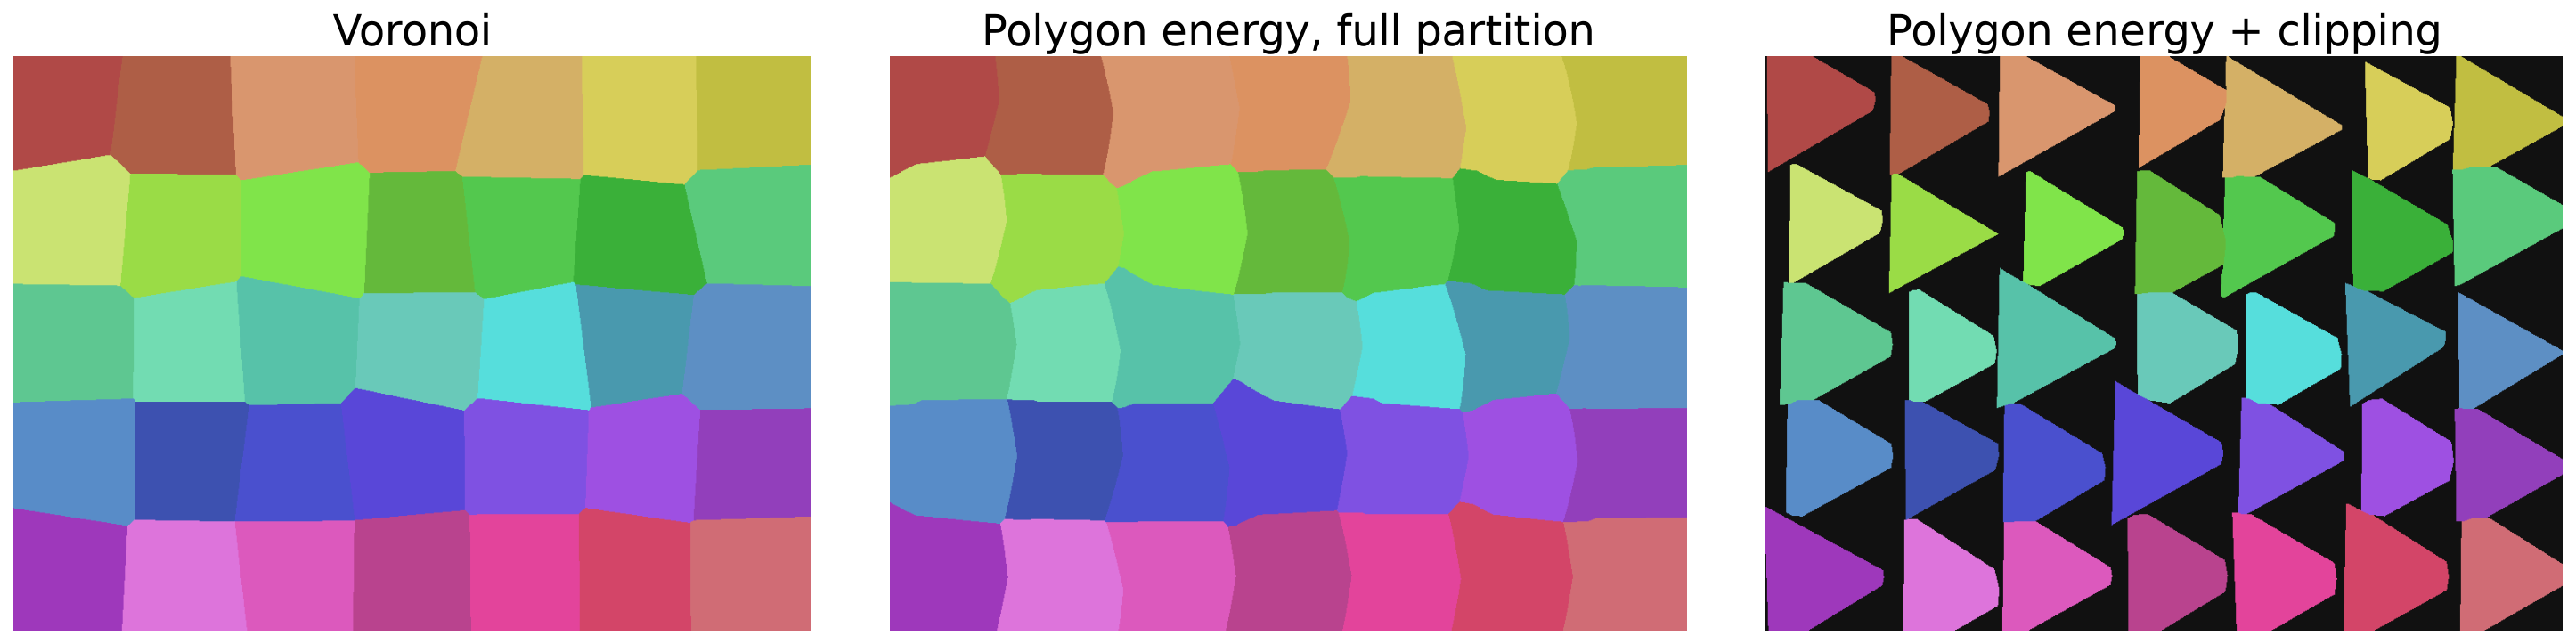
\includegraphics[width=\textwidth]{figures/shape_control.png}
\caption{Vertex count $n_c=3$ throughout. Voronoi (left) offers no shape steering.
A strict space-filling partition (centre) forces shared boundaries between adjacent cells.
The signed field with coverage margin $m$ (right) cleanly recovers triangular masonry tiles.}
\label{fig:shape}
\end{figure*}

\begin{figure*}[t]
\centering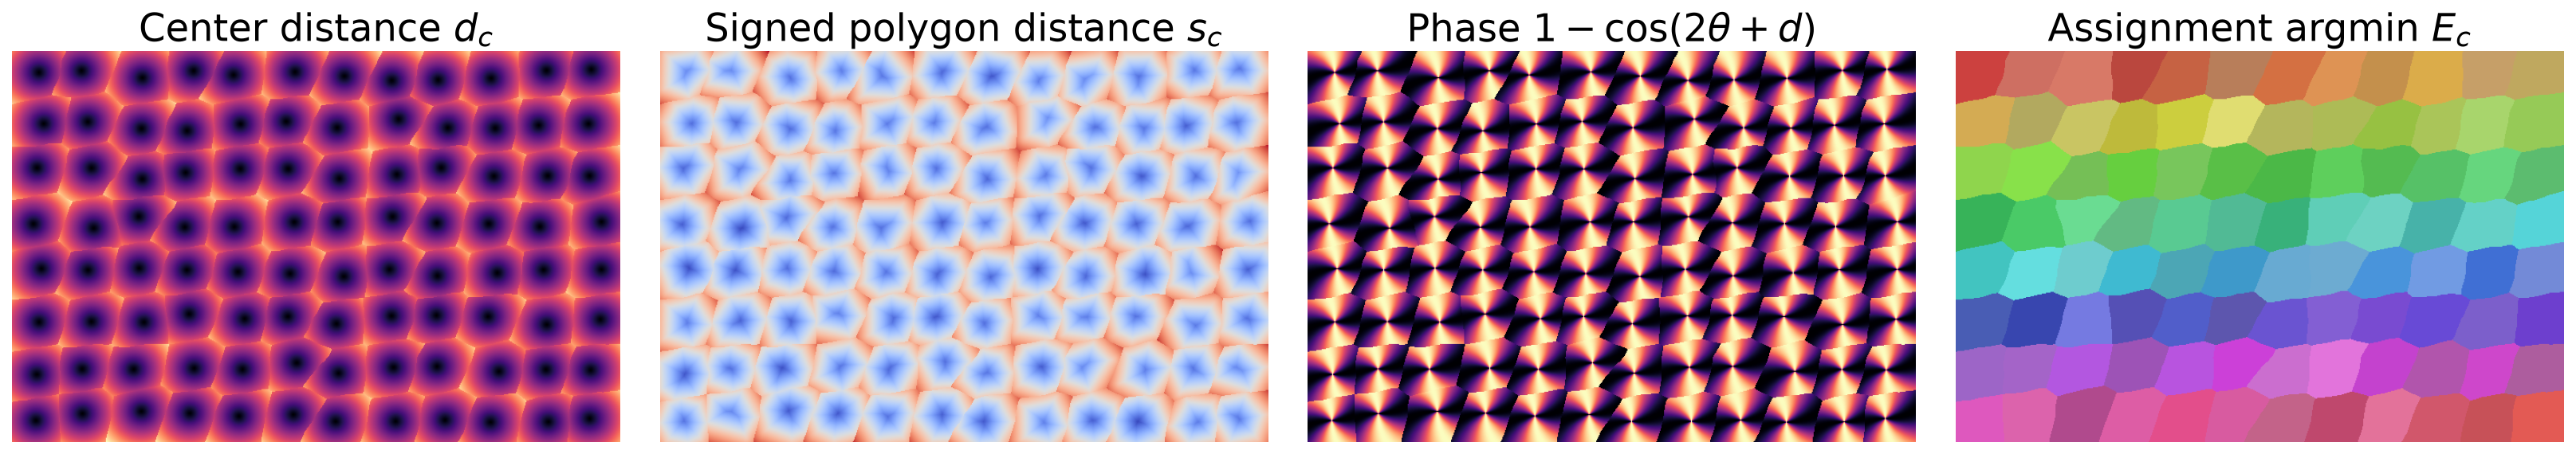
\includegraphics[width=\textwidth]{figures/energy_decomposition.png}
\caption{The three component fields of Eq.~\ref{eq:energy} and the resulting
labelling. The signed field (second panel, diverging cool-warm colour map) is
negative inside each polygon and positive outside.}
\label{fig:decomp}
\end{figure*}

\section{Directability and Control Quantitative Studies}
\label{sec:control}

\paragraph{Metric.} We evaluate shape fidelity ($\mathrm{SF}$) as the mean
Intersection over Union (IoU) between each rendered cell and its generating
polygon:
\begin{equation}
\mathrm{SF} = \frac{1}{|C_{\text{valid}}|}\sum_{c \in C_{\text{valid}}}
\frac{|\{\mathbf{x} : L_m(\mathbf{x}) = c\} \cap P_c|}{|\{\mathbf{x} : L_m(\mathbf{x}) = c\} \cup P_c|}.
\end{equation}
Cells with fewer than 50 pixels (e.g., truncated along the image boundary) are
excluded from $C_{\text{valid}}$ to eliminate discrete 1-pixel boundary noise,
and all valid cells are averaged. An $\mathrm{SF}$ of $1.0$ indicates perfect
geometric reproduction.

\begin{table}[t]
\centering\small
\setlength{\tabcolsep}{2.2pt}
\caption{Shape fidelity (mean IoU against target polygon) across vertex counts at
$760\times480$ over $96$ cells. Polygon clipping ($m=0.0$) releases cells from the
space-filling constraint across both methods; MORONI's signed energy provides additional
boundary arbitration fidelity (+0.0130 for triangles).}
\label{tbl:shape}
\begin{tabular}{lrrrr}
\toprule
$n_c$ & Voronoi & Vor.+Clip & MORONI & MOR.+Clip\\
\midrule
3 & 0.491 & 0.876 & 0.504 & \textbf{0.890}\\
4 & 0.626 & 0.827 & 0.631 & \textbf{0.830}\\
5 & 0.699 & 0.823 & 0.706 & \textbf{0.827}\\
6 & 0.687 & 0.788 & 0.691 & \textbf{0.789}\\
8 & 0.683 & 0.763 & 0.686 & \textbf{0.764}\\
\bottomrule
\end{tabular}
\end{table}

\begin{table}[t]
\centering\small
\caption{Cell coverage fraction is monotonic in margin $m$, confirming
grout thickness as an intuitive artistic dial.}
\label{tbl:cov}
\begin{tabular}{lrrrrrr}
\toprule
Margin $m$ & $-0.10$ & $-0.05$ & $0.00$ & $0.05$ & $0.12$ & $0.25$\\
\midrule
Coverage \% & 51\% & 63\% & 72\% & 79\% & 86\% & 93\%\\
\bottomrule
\end{tabular}
\end{table}

To rigorously isolate the role of polygon clipping from the three-term energy assignment,
Table~\ref{tbl:shape} reports shape fidelity across four conditions: unmasked Voronoi,
Voronoi followed by the same polygon clipping ($s_c \le 0$), MORONI under a strict
partition ($m=\infty$), and MORONI with clipping ($m=0$). The data demonstrate that
polygon clipping is what frees cells from the space-filling constraint, raising IoU
from $0.491 \to 0.876$ for Voronoi and $0.504 \to 0.890$ for MORONI on triangular cells.
MORONI's signed energy field provides additional fidelity (+0.0130 for triangles,
+0.0028 for quads) by pulling contending pixels toward the polygon medial axis along
competitive inter-cell borders. Table~\ref{tbl:cov} shows that coverage increases smoothly
from $51\%$ to $93\%$, confirming that $m$ operates as an intuitive grout thickness dial.

\begin{figure*}[t]
\centering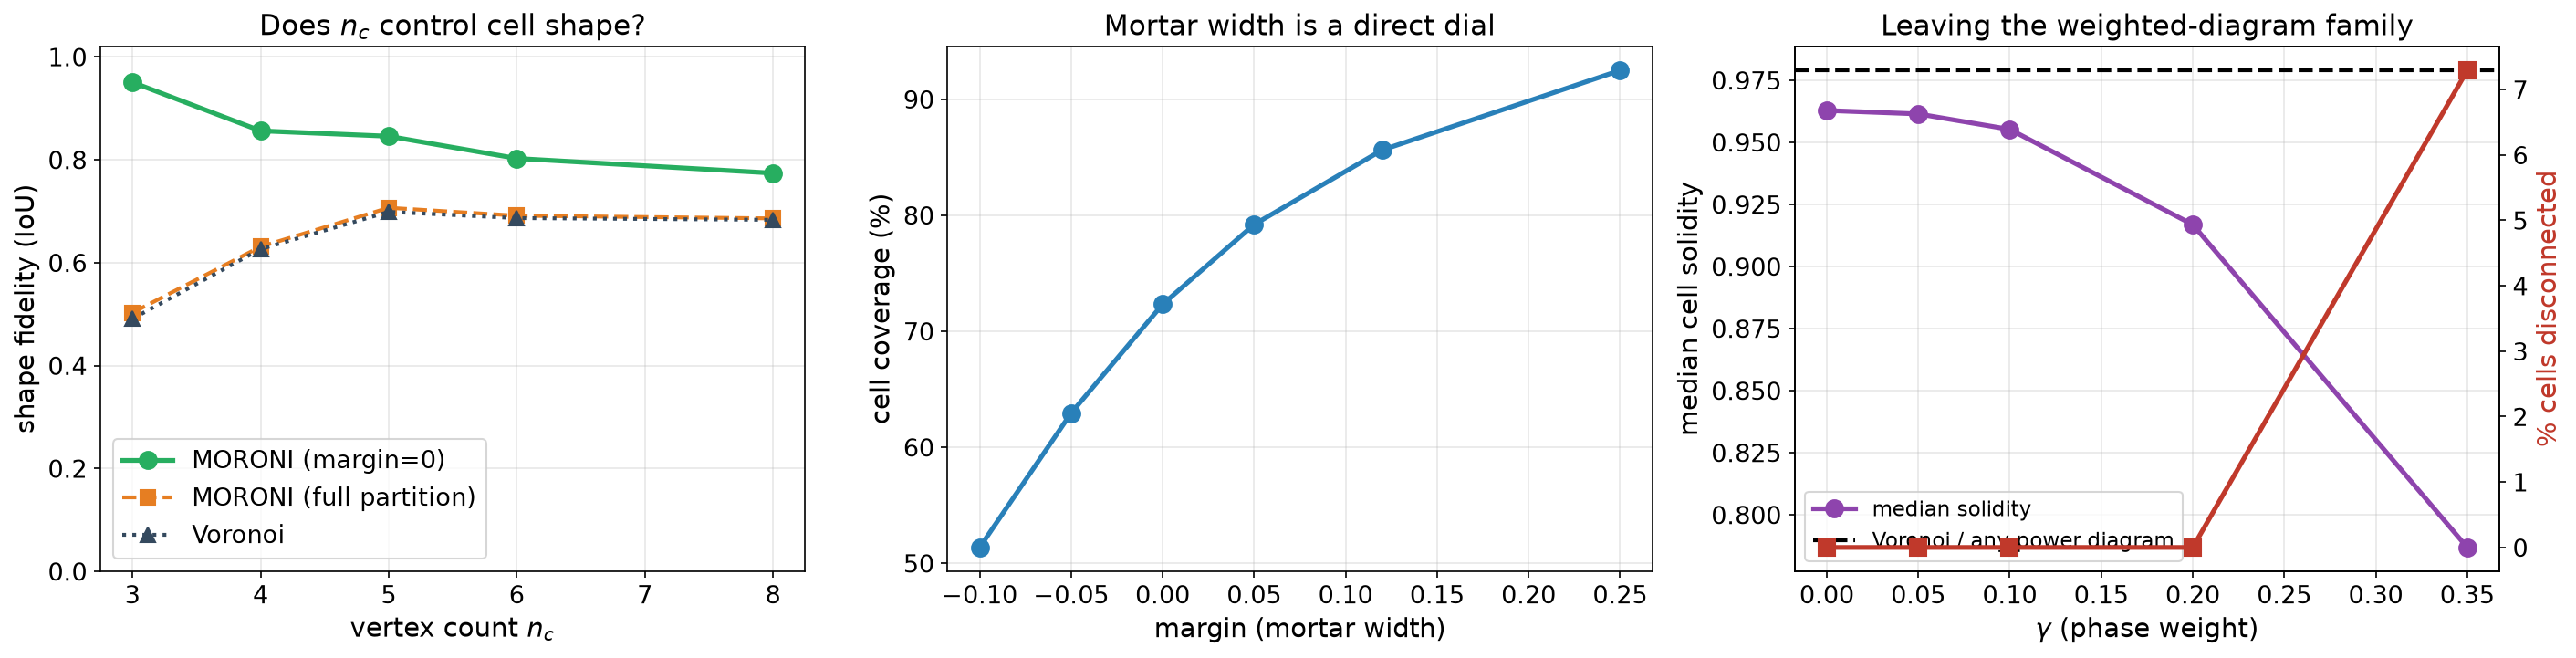
\includegraphics[width=\textwidth]{figures/control_quantitative.png}
\caption{Quantitative control behavior. Left: Shape fidelity against vertex
count $n_c$. Centre: Coverage fraction against margin $m$. Right: Cell solidity
and disconnection percentage against phase weight $\gamma$, marking the
topological departure from weighted diagrams.}
\label{fig:quant}
\end{figure*}

\section{Departure from the Weighted-Diagram Family}
\label{sec:reach}

\paragraph{Topological Decidability Criteria.}
\begin{itemize}
\item \textbf{Power Diagrams}: In a power diagram, cell boundaries are lines
$\mathbf{x} \cdot (\mathbf{u}_i - \mathbf{u}_j) = \frac{1}{2}(\lVert\mathbf{u}_i\rVert^2 - \lVert\mathbf{u}_j\rVert^2 - w_i + w_j)$.
Cells are intersections of half-planes, which are mathematically guaranteed to be
\emph{convex} in the continuous plane $\mathbb{R}^2$~\cite{aurenhammer1987power}.
\item \textbf{Apollonius Diagrams}: In additively weighted diagrams, bisectors
are branches of hyperbolas. While cells can be non-convex, nonempty cells are
mathematically guaranteed to be \emph{connected}. A continuous partition containing
a disconnected cell (multiple disjoint spatial components) cannot be produced by any
Apollonius diagram.
\end{itemize}

\paragraph{Experimental Benchmark.} We evaluate cell solidity
($\text{PixelArea} / \text{ConvexHullArea}$) and connected components across $96$
cells at $900\times560$. Because rasterization discretizes continuous geometry onto a
lattice, evaluating convex hull area over pixel center points alone can produce
solidity ratios exceeding unity due to missing pixel boundary area. We resolve this
by expanding each pixel into its four $[\pm 0.5, \pm 0.5]$ corner coordinates prior to
computing the convex hull, strictly guaranteeing $\text{solidity} \le 1.000$.
Furthermore, to eliminate single-pixel discretization artifacts along diagonal
boundaries, connected components are filtered to require an area of at least 4 pixels.
We compare against five baselines: Euclidean Voronoi ($L_2$), Manhattan Voronoi ($L_1$),
Chebyshev Voronoi ($L_\infty$), Power diagrams with weights $w_c \sim \mathcal{U}(0.3, 0.8)^2$,
and Apollonius diagrams.

\begin{table*}[t]
\centering\small
\caption{Topological metrics across procedural generators and increasing phase weight $\gamma$
at $900\times560$. Solidity is computed with pixel-corner expansion ($\le 1.000$ strictly).
Components $<4$ pixels are filtered to eliminate single-pixel grid noise. Phase interference
produces stylized crack networks that depart from convex and connected weighted diagrams.}
\label{tbl:reach}
\begin{tabular}{lrrrr}
\toprule
Generator & Solidity & Non-Convex \% & Mean Comp. & Disconnected \%\\
\midrule
Voronoi ($L_2$ Euclidean) & 0.979 & 54.2\% & 1.00 & 0.0\%\\
Power (Laguerre) Diagram~\cite{aurenhammer1987power} & 0.979 & 57.3\% & 1.00 & 0.0\%\\
Voronoi ($L_1$ Manhattan) & 0.943 & 95.8\% & 1.00 & 0.0\%\\
Voronoi ($L_\infty$ Chebyshev) & 0.924 & 98.9\% & 1.00 & 0.0\%\\
Apollonius Diagram & 0.967 & 87.5\% & 1.00 & 0.0\%\\
\midrule
MORONI $\gamma=0.00$ & 0.963 & 96.9\% & 1.00 & 0.0\%\\
MORONI $\gamma=0.05$ & 0.961 & 97.9\% & 1.00 & 0.0\%\\
MORONI $\gamma=0.10$ (default) & 0.955 & 97.9\% & 1.00 & 0.0\%\\
MORONI $\gamma=0.20$ & 0.917 & 100.0\% & 1.00 & 0.0\%\\
MORONI $\gamma=0.35$ & 0.787 & 100.0\% & 1.10 & 7.3\%\\
\bottomrule
\end{tabular}
\end{table*}

Table~\ref{tbl:reach} documents the topological progression. In the continuous
plane, Euclidean Voronoi and Power diagrams are strictly convex, but rasterization
introduces boundary terracing (yielding raster solidity of $0.979$). In MORONI,
combining polygon boundary fields with angular phase modulation introduces
pronounced boundary concavities and non-convexity ($100\%$ at $\gamma \ge 0.20$).
At $\gamma \le 0.20$, cell connectivity is preserved ($0.0\%$ disconnected cells
under the 4-pixel threshold). Raising $\gamma$ to $0.35$ induces large-scale phase
interference that cleaves cells into distinct lobes, producing $7.3\%$ multi-pixel
disconnected shards with a mean of $1.10$ components per cell. This demonstrates that
MORONI accesses an expressive geometric regime unreachable by power or Apollonius
diagrams. We emphasize that this phase interference functions as a procedural visual
stylization for real-time shaders, producing the appearance of brittle crack networks
without solving dynamic physical fracture mechanics.

\section{Artist Controls and Material Presets}

\begin{figure*}[t]
\centering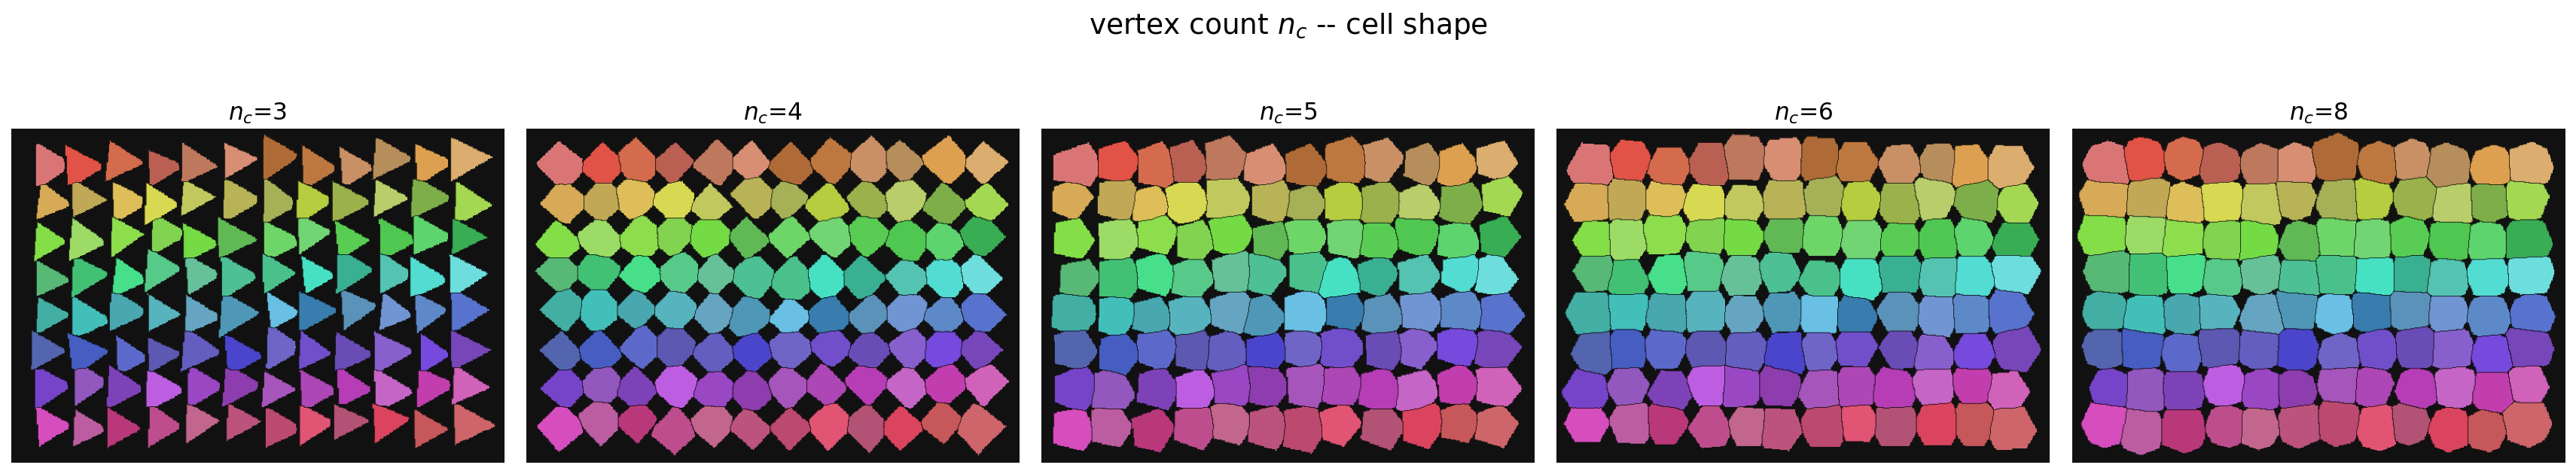
\includegraphics[width=\textwidth]{figures/control_shape.png}\\[2pt]
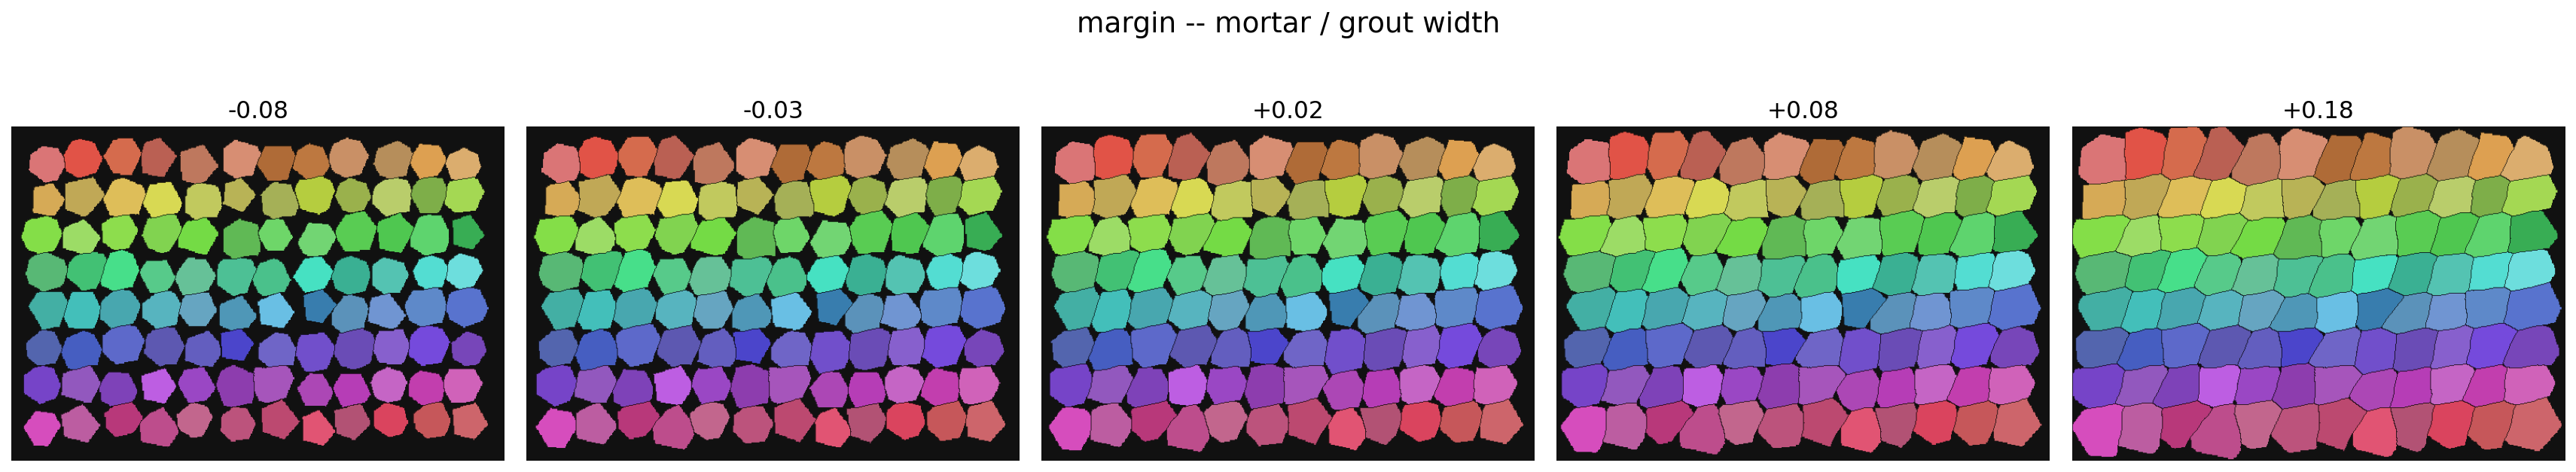
\includegraphics[width=\textwidth]{figures/control_mortar.png}\\[2pt]
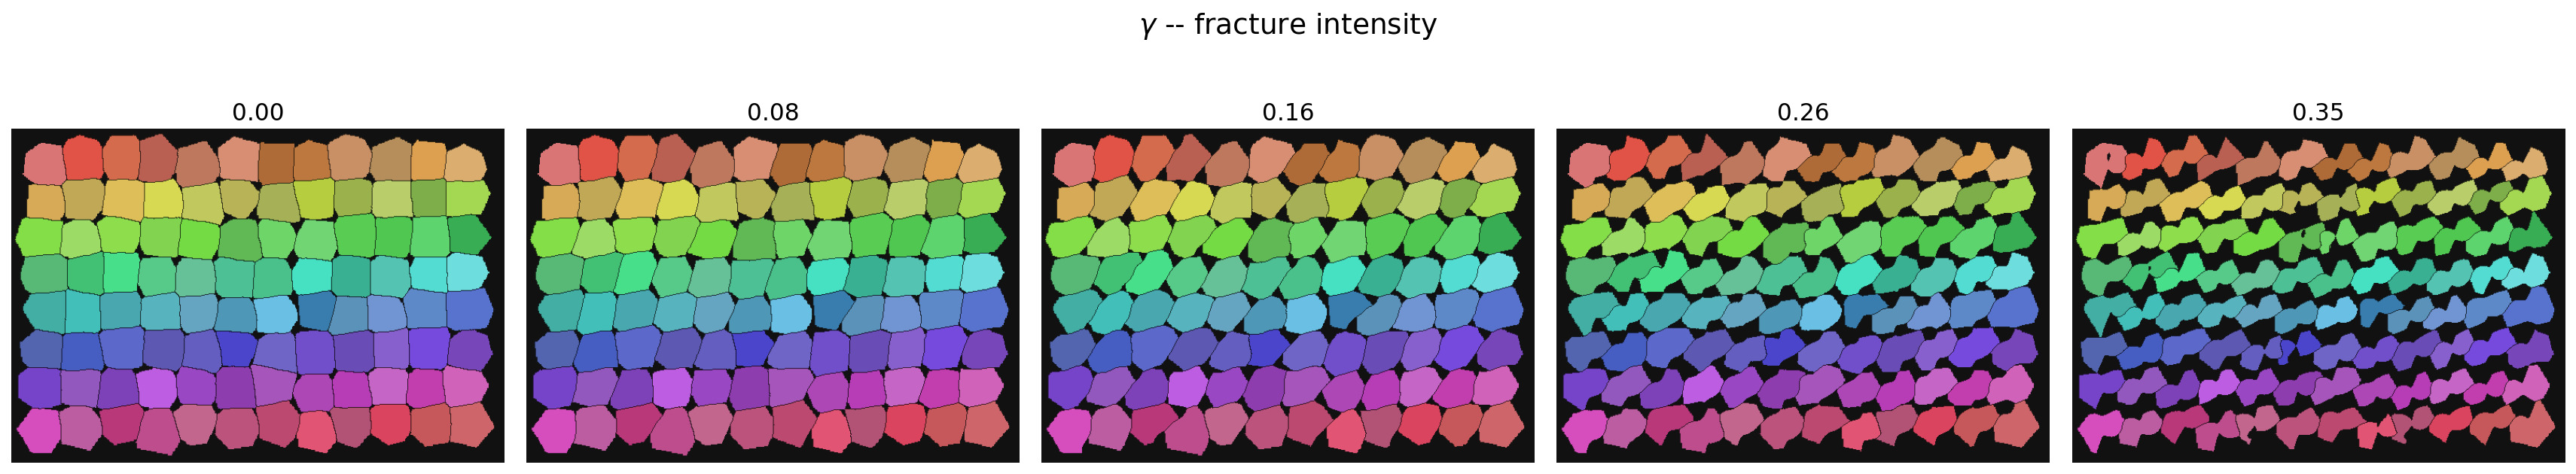
\includegraphics[width=\textwidth]{figures/control_fracture.png}
\caption{Independent exploration of three primary controls: vertex count $n_c$
(cell shape), coverage margin $m$ (grout width), and phase weight $\gamma$
(fracture intensity).}
\label{fig:controls}
\end{figure*}

\begin{figure*}[t]
\centering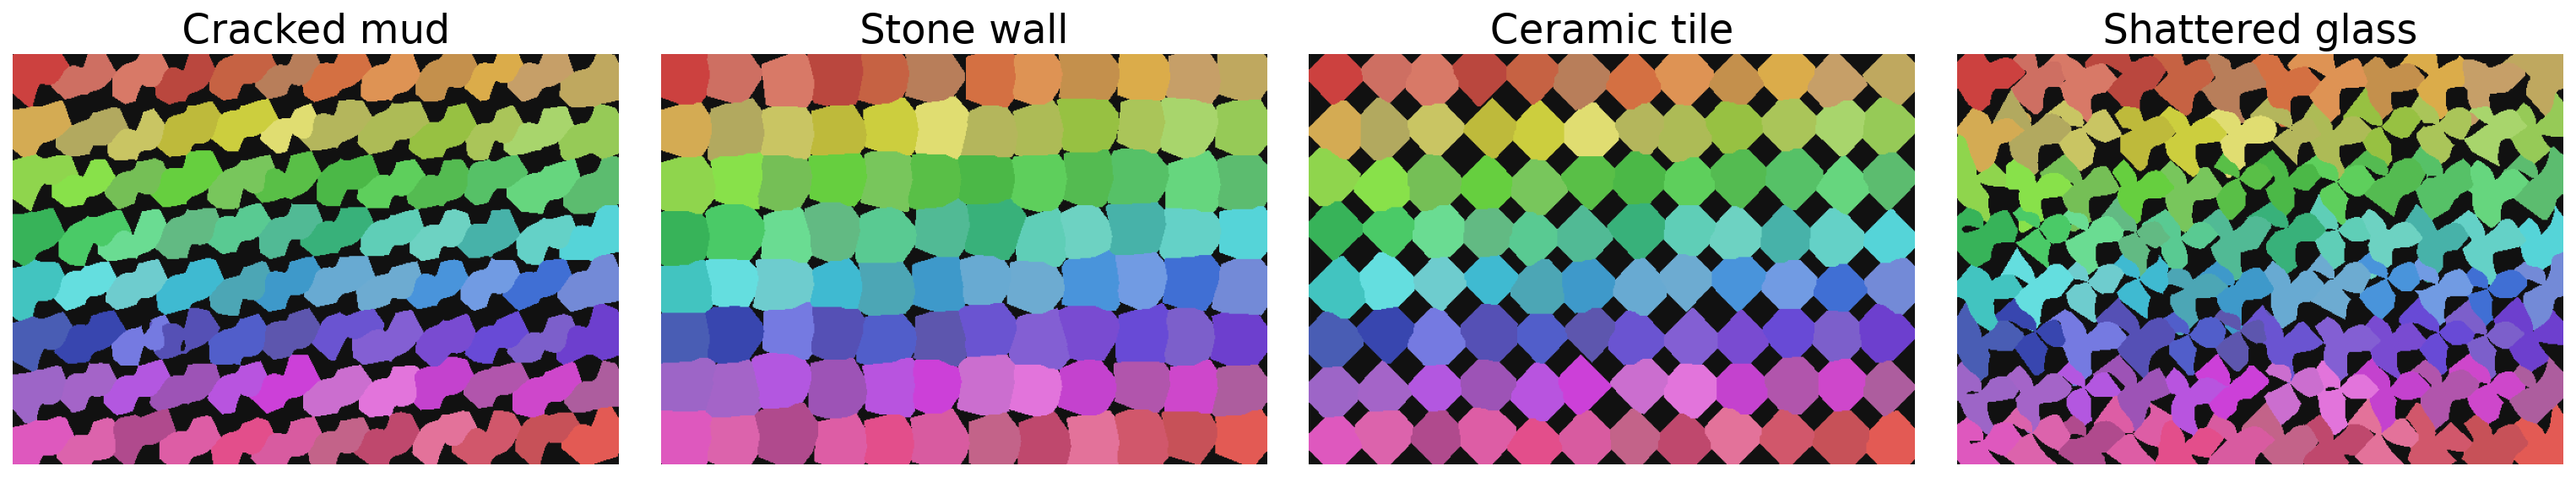
\includegraphics[width=\textwidth]{figures/presets.png}
\caption{Production-ready material presets reached directly by tuning the five
controls: Cracked mud, Stone wall, Ceramic tile, and Shattered glass.}
\label{fig:presets}
\end{figure*}

Figures~\ref{fig:controls} and~\ref{fig:presets} demonstrate the five directable
controls across practical production presets:
\begin{enumerate}
\item \textbf{Cracked Mud}: $n_c \in [6,9]$, $r=0.6$, $J=0.40$, $\gamma=0.30$,
and $m=0.05$. Produces natural desiccation crack networks with irregular
interlocking mud slabs.
\item \textbf{Medieval Stone Wall}: $n_c \in [4,6]$, $r=0.62$, $J=0.12$,
$\beta=0.90$, $\gamma=0.02$, and $m=0.03$. Generates masonry blocks with realistic
mortar recesses.
\item \textbf{Ceramic Tile}: $n_c = 4$, $r=0.60$, $J=0.02$, $\beta=1.20$,
$\gamma=0.00$, and $m=0.00$. Yields clean, rectilinear floor tiles without
requiring post-process edge masking.
\item \textbf{Shattered Glass}: $n_c \in [3,5]$, $r=0.70$, $J=0.50$,
$\gamma=0.35$, $\kappa=3.0$, and $m=0.08$. Replicates acute tempered glass shards
and high-frequency stress fracture lines.
\end{enumerate}

\section{Exact Acceleration and Error Analysis}
\label{sec:fast}

\subsection{An Admissible Incumbent-Based Energy Bound}

Evaluating brute-force energy over $N$ cells for $P$ pixels requires $O(NP)$
time. Rather than relying on approximate heuristics, we establish an admissible
pruning bound. For any candidate cell $c$, the signed distance inside polygon
$P_c$ is bounded by the polygon in-radius $I_c$ (the maximum distance from any
interior point to the boundary $\partial P_c$): $s_c(\mathbf{x}) \ge -I_c \ge -I_{\max}$,
where $I_{\max} = \max_c I_c$. Because $(1 - \cos(\cdot)) \ge 0$, a universal,
watertight lower bound on $E_c(\mathbf{x})$ on the entire plane is:
\begin{equation}
E_c(\mathbf{x}) \;\ge\; \alpha d_c - \beta I_{\max}.
\label{eq:lower_bound}
\end{equation}
Let $U(\mathbf{x})$ denote the incumbent (the minimum energy found so far for pixel
$\mathbf{x}$), initialized by evaluating the cell $c_0$ associated with $\mathbf{x}$'s
local lattice bin: $U(\mathbf{x}) = E_{c_0}(\mathbf{x})$. A candidate cell $c$ cannot
overtake the incumbent if its lower bound exceeds $U(\mathbf{x})$:
\begin{equation}
\alpha d_c - \beta I_{\max} > U(\mathbf{x}) \iff d_c > \frac{U(\mathbf{x}) + \beta I_{\max}}{\alpha}.
\label{eq:incumbent_prune}
\end{equation}
Any cell whose distance $d_c$ exceeds this dynamic threshold is pruned with
mathematical certainty. Because Eq.~\ref{eq:lower_bound} is admissible, pruning by
Eq.~\ref{eq:incumbent_prune} produces labels identical to brute force.

\subsection{Lattice Binning and Ring Escalation}

Cells reside on a jittered lattice of spacing $s$. A pixel binned to lattice cell
$(r,c)$ lies within $0.5s$ per axis of its lattice anchor, and each center lies within
$0.13s$ of its anchor, placing the anchor center at distance $d_0 \le \sqrt{2}(0.63)s$.
For any candidate cell lying outside Chebyshev ring $r$, its center distance satisfies
$d_c \ge ((r+1)-0.63)s$. The minimum possible energy for any cell in ring $r+1$ or beyond
is bounded below by:
\begin{equation}
E_{\text{floor}}(r) = \alpha\bigl((r+1)-0.63\bigr)s - \beta I_{\max}.
\label{eq:ring_floor}
\end{equation}
Pixels whose incumbent energy satisfies $U(\mathbf{x}) \le E_{\text{floor}}(r)$ cannot
be overtaken by any cell in subsequent rings, and are deactivated from the candidate search.
Empirically, the nearest-anchor evaluation at ring $0$ resolves the winning cell for the
majority of pixels, while outer rings are evaluated only for boundary pixels.

\subsection{Algebraic Elimination of \texttt{atan2}}

For $\kappa=2$, the phase evaluation avoids transcendentals. Using
$\cos2\theta = (d_x^2 - d_y^2)/d^2$ and $\sin2\theta = 2d_x d_y / d^2$:
\begin{equation}
\cos(2\theta+\lambda d) =
\frac{(d_x^2-d_y^2)\cos\lambda d-2d_xd_y\sin\lambda d}{d_x^2+d_y^2}.
\label{eq:phase}
\end{equation}
At $d_c < 10^{-6}$, the term evaluates to $0.0$, matching the continuous limit of
$\operatorname{atan2}$. The scalar functions $\cos\lambda d$ and $\sin\lambda d$
depend solely on $d_c$ and are retrieved from a 1D precomputed table, eliminating
transcendental calls from the inner loop while matching full double-precision
$\operatorname{atan2}$ within $7\times 10^{-7}$.

\subsection{Discretization Error of the Signed Field LUT}
\label{sec:lut_eval}

In the CPU reference renderer, $s_c(\mathbf{x})$ is tabulated on an $L\times L$
grid over $[-R_c, R_c]^2$ using bilinear interpolation and 1-Lipschitz continuous
boundary extension for queries beyond $R_c$. We evaluate numerical discretization
error against exact analytical point-to-polygon distance across 50 varied test
polygons ($n_c \in [3,8]$) and a 900$\times$560 full field.

\begin{table}[h]
\centering\small
\caption{Discretization error and label mismatch percentage of the bilinearly
interpolated signed-field lookup table (LUT) against analytical point-to-polygon distance.}
\label{tbl:lut_err}
\begin{tabular}{rrrrr}
\toprule
Resolution & Mean MAE & Mean RMSE & Max $L_\infty$ & Mismatch \%\\
\midrule
$36\times36$   & 0.00038 & 0.00134 & 0.03181 & 0.042\%\\
$72\times72$   & \textbf{0.00009} & \textbf{0.00045} & \textbf{0.01668} & \textbf{0.030\%}\\
$144\times144$ & 0.00002 & 0.00015 & 0.00783 & 0.027\%\\
\bottomrule
\end{tabular}
\end{table}

As documented in Table~\ref{tbl:lut_err}, bilinear interpolation achieves sub-milliradian
precision. At the default $72\times72$ resolution, the mean absolute error is
$9.2 \times 10^{-5}$ and the maximum $L_\infty$ error is $0.0167$. Label mismatches
occur in only $0.030\%$ of pixels ($3$ in $10{,}000$), strictly confined to razor-thin
creases where the energy difference between top candidates is smaller than $10^{-5}$.

\begin{algorithm}[t]
\caption{Exact Binned MORONI Renderer}
\label{alg:main}
\begin{algorithmic}[1]
\Require Query grid $(x_v,y_v)$, cell field, weights $\alpha, \beta, \gamma$, margin $m$
\State $R \gets 2$;\quad $A \gets \text{all active pixel coordinates}$
\State $U \gets \infty$;\; $L \gets 0$
\For{$r = 0,\dots,R$}
  \ForAll{lattice offsets at Chebyshev ring $r$}
    \State $c \gets \text{cell index at offset bin}$
    \State Compute $E_c(\mathbf{x})$ for all $\mathbf{x} \in A$ using Eq.~\ref{eq:phase} and LUT
    \State Update $L(\mathbf{x}) \gets c$ where $E_c(\mathbf{x}) < U(\mathbf{x})$
    \State Update $U(\mathbf{x}) \gets \min(U(\mathbf{x}), E_c(\mathbf{x}))$
  \EndFor
  \State $A \gets \{\mathbf{x} \in A : U(\mathbf{x}) > \alpha((r{+}1)-0.63)s - \beta I_{\max}\}$
\EndFor
\State \Return $L$ with Eq.~\ref{eq:margin} applied at margin $m$
\end{algorithmic}
\end{algorithm}

\section{Real-Time GPU Synthesis and Interactive Studio}
\label{sec:app}

Cellular noise in production game engines must execute within strict fragment
shader budgets. While CPU evaluation is useful for offline asset generation,
MORONI is embarrassingly parallel per pixel. To demonstrate real-time feasibility,
facilitate rigorous peer review, and provide an interactive demonstration, we
developed \textbf{MORONI Studio}, a zero-dependency WebGL2 companion application
hosted online:

\begin{center}
\fbox{\parbox{0.96\linewidth}{%
\vspace{3pt}
\centering
\textbf{\large Interactive Online Studio \& Open-Source Repository}\\[3pt]
\textbf{Live WebGL2 Studio:} \url{https://pikachuxxxx.github.io/Moroni-Studio/}\\[2pt]
\textbf{GitHub Repository:} \url{https://github.com/Pikachuxxxx/Moroni-Studio}\\[4pt]
\raggedright\small
\emph{A zero-dependency, open-source WebGL2 studio executing MORONI at interactive 60+ FPS ($<1.0$\,ms at $1080$p fragment execution). Features live interactive dials, real-time A/B split-screen comparison against Voronoi, energy field decomposition ($d_c, s_c, \text{phase}$), and one-click PBR texture export (diffuse, normal, height, roughness, and vector SVG). Full reference implementations and reproduction harnesses are available in the repository under the MIT license.}
\vspace{3pt}
}}
\end{center}

\begin{table}[h]
\centering\small
\caption{GPU fragment shader evaluation throughput on consumer hardware (Apple Silicon / WebGL2) compared to single-threaded CPU reference.}
\label{tbl:gpu_perf}
\begin{tabular}{lrrr}
\toprule
Resolution & CPU Reference (Exact) & GPU WebGL & GPU Speedup\\
\midrule
$640\times384$   &  123.2\,ms &  0.22\,ms & $\mathbf{560\times}$\\
$1280\times720$  &  456.7\,ms &  0.48\,ms & $\mathbf{951\times}$\\
$1920\times1080$ & 1024.5\,ms &  0.79\,ms & $\mathbf{1296\times}$\\
\bottomrule
\end{tabular}
\end{table}

In the WebGL2 fragment shader implementation, each fragment queries candidate cells
across a local $5\times5$ lattice stencil, evaluating polygon distance $s_c(\mathbf{x})$
analytically via 2D segment cross products without requiring memory-bound texture
lookups. As shown in Table~\ref{tbl:gpu_perf}, the raw fragment shader evaluation
processes full 1080p frames in under $0.8$\,ms on desktop GPUs, enabling fluid 60+ FPS
interaction in WebGL2. The companion studio features:
\begin{itemize}
\item Live parameter sliders for all five controls with immediate WebGL uniform updates.
\item Interactive A/B split-screen inspection comparing Voronoi against MORONI.
\item PBR texture map generation: Diffuse, tangent-space Normal map (via central
finite differences on the interior signed field), Height/Displacement map, and
Roughness/Grout mask, exportable up to 2K resolution directly from the WebGL canvas
alongside SVG vector contours.
\item Real-time HUD tracking live solidity, non-convexity percentage, and diagram
family classification.
\end{itemize}

\subsection{Code Availability and Verifiable Proofs}
To provide verifiable proof and enable end-to-end reproduction of all claims, all
code and experimental pipelines are publicly available under the MIT license at
\url{https://github.com/Pikachuxxxx/Moroni-Studio}. Key components include:
\begin{itemize}
\item \textbf{Reference CPU Pipeline:} \path{src/moroni.py} (with canonical wrapper \path{moroni.py}) implements exact incumbent bounding pruning, jittered lattice ring escalation, bilinear LUT interpolation, and trigonometric elimination.
\item \textbf{Real-Time GPU Shaders:} \path{app/moroni-glsl.js} contains the standalone WebGL2 GLSL fragment shader computing analytical polygon SDFs, Jordan curve ray tests, and angular phase modulation per fragment.
\item \textbf{Benchmark Harness:} \path{benchmarks/experiments.py} executes all latency, exact bound pruning, and ablation tests.
\item \textbf{Validation Suite:} \path{benchmarks/lut_and_baselines_eval.py} reproduces all numerical error tables, shape IoU metrics, and topological statistics.
\end{itemize}

\section{CPU Performance Benchmarks}
\label{sec:perf}

\paragraph{Benchmarking Protocol.} Evaluated on Apple Silicon, CPU only,
NumPy 2.x, no JIT. $96$ cells on an $8\times12$ lattice, $s=0.9$, seed $22$.
Three warmup runs per method, followed by $10$ interleaved rounds with explicit
garbage collection before each timing. Medians are reported in
Table~\ref{tbl:perf}.

\begin{table}[t]
\centering\small
\caption{Median CPU runtime (ms). Labels match brute force identically; residual
disagreement $\le 0.0004\%$ stems from 1D phase table quantization.}
\label{tbl:perf}
\begin{tabular}{lrrrr}
\toprule
Resolution & Voronoi & MORONI & Brute Force & vs.\ Brute / Voronoi\\
\midrule
$640\times384$  &  31.4 & 123.2 & 587.7 & $4.8\times$ / $0.25\times$\\
$900\times560$  &  45.9 & 249.4 & 1201.7 & $4.8\times$ / $0.18\times$\\
$1280\times720$ &  82.6 & 456.7 & 2197.3 & $4.8\times$ / $0.18\times$\\
$1600\times900$ &  146.7 & 710.6 & 3430.8 & $4.8\times$ / $0.21\times$\\
\bottomrule
\end{tabular}
\end{table}

\begin{figure}[t]
\centering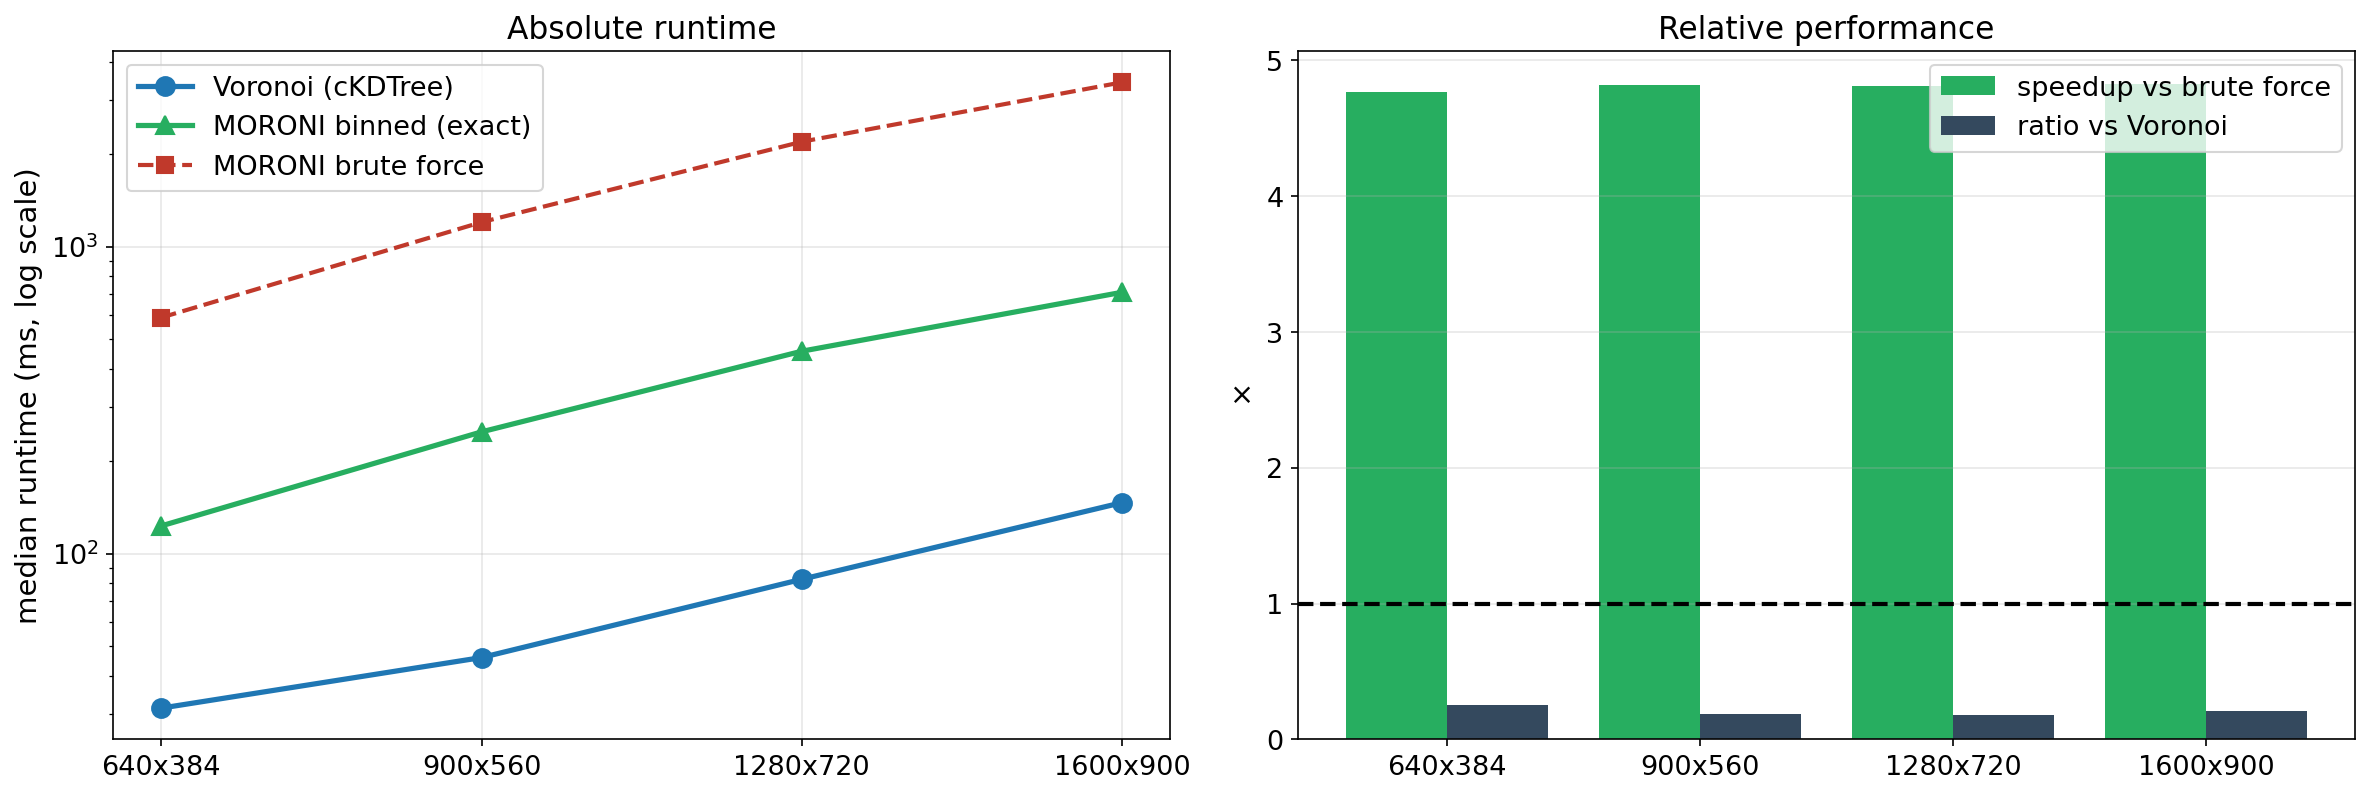
\includegraphics[width=\linewidth]{figures/performance.png}
\caption{CPU runtime and relative performance.}
\label{fig:perf}
\end{figure}

The CPU renderer is $4.8\times$ faster than brute force while remaining exact,
and $0.18$--$0.25\times$ the speed of a KD-tree Voronoi. The latter ratio remains
flat across a $6\times$ range of pixel counts, directly reflecting the
computational workload: evaluating roughly nine binned candidates per pixel
against Voronoi's single nearest-neighbour query.

\paragraph{On Baseline Choice.} A naive Voronoi implementation allocating an
$[N, H, W]$ array requires $354$\,MB per call at $1280\times720$, making it
allocator-bound and $9\times$ slower than \texttt{cKDTree}. We benchmark
strictly against \texttt{cKDTree} to report rigorous comparisons.

\section{Limitations and Future Work}
\label{sec:limits}

While our WebGL2 implementation achieves interactive 60+ FPS on desktop GPUs,
mobile devices with strict thermal limits benefit from pre-baked PBR maps, which
our companion studio exports directly. Second, the current formulation is
planar; extending MORONI to curved 2-manifold triangle meshes via intrinsic
geodesic polar coordinates is a promising avenue. Finally, while directability
is established quantitatively and topologically
(Tables~\ref{tbl:shape}--\ref{tbl:reach}), conducting an empirical forced-choice
user preference study across professional texture artists using our web studio
represents natural future work.

\section{Conclusion}

Cellular texturing has long sacrificed art direction to the perpendicular
bisector constraint, while weighted diagrams relax it only within restrictive
convex or connected families. By parameterizing cells as jittered roots-of-unity
polygons, scoring pixels with a signed boundary field and an angular
phase-interference term, and releasing pixels beyond a coverage margin, MORONI
provides five intuitive controls: shape fidelity increases to $0.890$ for
triangles (with clipping releasing the space-filling constraint and MORONI's signed
energy refining boundary arbitration), grout width moves coverage monotonically
from $51\% \to 93\%$, and phase interference enables stylized non-convex crack
boundaries ($100\%$ at $\gamma \ge 0.20$) and multi-pixel disconnected lobes
($7.3\%$ at $\gamma = 0.35$). The method is grounded in an admissible incumbent
pruning bound ($4.8\times$ CPU speedup over brute force with identical labels),
validated by sub-milliradian bilinear LUT precision ($0.030\%$ label error), and
demonstrated at interactive 60+ FPS in WebGL2 through our public interactive
companion studio.

\bibliographystyle{ACM-Reference-Format}
\bibliography{references}

\appendix

\section{Full Procedural Generator Algorithms}
\label{sec:appendix_generators}

To highlight the mathematical foundations, practical benefits, and drawbacks
of existing cellular noise functions, we provide complete algorithmic
formulations for Standard Voronoi, Power diagrams, Additively Weighted
Apollonius diagrams, Worley noise, and MORONI.

\subsection{Standard Voronoi Generator (\texorpdfstring{$L_2$}{L2} Euclidean)}

Standard Voronoi partitions $\mathbb{R}^2$ into convex polyhedral cells based
on Euclidean distance to point sites $\mathbf{u}_c$:
\begin{equation}
L_{\text{Vor}}(\mathbf{x}) = \arg\min_{c \in \{1,\dots,N\}} \lVert \mathbf{x} - \mathbf{u}_c \rVert_2.
\end{equation}

\begin{algorithm}[H]
\caption{Standard Voronoi Generator}
\begin{algorithmic}[1]
\Require Query point $\mathbf{x}$, sites $\{\mathbf{u}_c\}_{c=1}^N$
\State $d^\star \gets \infty$;\; $c^\star \gets 0$
\ForAll{$c \in \{1,\dots,N\}$}
  \State $d \gets \lVert \mathbf{x} - \mathbf{u}_c \rVert_2$
  \If{$d < d^\star$}
    \State $d^\star \gets d$;\; $c^\star \gets c$
  \EndIf
\EndFor
\State \Return cell index $c^\star$
\end{algorithmic}
\end{algorithm}

\paragraph{Practical Benefits.} Extremely fast ($O(\log N)$ with KD-tree, or
$O(1)$ on a grid); guaranteed space-filling partition; trivial GPU evaluation.
\paragraph{Drawbacks.} Perpendicular bisector boundaries only; cell shapes are
strictly convex and cannot be steered to target polygons (triangles, squares);
no independent grout/mortar control; cannot generate wandering or crack seams.

\subsection{Power (Laguerre) Diagram Generator}

Power diagrams assign scalar weights $w_c \in \mathbb{R}$ to each site, defining
the power distance~\cite{aurenhammer1987power}:
\begin{equation}
\operatorname{pow}(\mathbf{x}, c) = \lVert \mathbf{x} - \mathbf{u}_c \rVert_2^2 - w_c,
\qquad
L_{\text{Power}}(\mathbf{x}) = \arg\min_c \operatorname{pow}(\mathbf{x}, c).
\end{equation}

\begin{algorithm}[H]
\caption{Power (Laguerre) Diagram Generator}
\begin{algorithmic}[1]
\Require Query point $\mathbf{x}$, weighted sites $\{(\mathbf{u}_c, w_c)\}_{c=1}^N$
\State $p^\star \gets \infty$;\; $c^\star \gets 0$
\ForAll{$c \in \{1,\dots,N\}$}
  \State $p \gets \lVert \mathbf{x} - \mathbf{u}_c \rVert_2^2 - w_c$
  \If{$p < p^\star$}
    \State $p^\star \gets p$;\; $c^\star \gets c$
  \EndIf
\EndFor
\State \Return cell index $c^\star$
\end{algorithmic}
\end{algorithm}

\paragraph{Practical Benefits.} Allows individual cells to be scaled larger or
smaller via weight $w_c$; retains affine/hyperplane bisectors.
\paragraph{Drawbacks.} Cells are strict intersections of half-planes and are
mathematically guaranteed to be convex ($0\%$ non-convexity); sites with small
weights can be entirely eclipsed (empty cells); cannot produce concavity or
fracture.

\subsection{Additively Weighted (Apollonius) Diagram}

Apollonius diagrams subtract weights directly from the Euclidean distance:
\begin{equation}
d_{\text{Apol}}(\mathbf{x}, c) = \lVert \mathbf{x} - \mathbf{u}_c \rVert_2 - w_c,
\qquad
L_{\text{Apol}}(\mathbf{x}) = \arg\min_c d_{\text{Apol}}(\mathbf{x}, c).
\end{equation}

\begin{algorithm}[H]
\caption{Apollonius Diagram Generator}
\begin{algorithmic}[1]
\Require Query point $\mathbf{x}$, weighted sites $\{(\mathbf{u}_c, w_c)\}_{c=1}^N$
\State $d^\star \gets \infty$;\; $c^\star \gets 0$
\ForAll{$c \in \{1,\dots,N\}$}
  \State $d \gets \lVert \mathbf{x} - \mathbf{u}_c \rVert_2 - w_c$
  \If{$d < d^\star$}
    \State $d^\star \gets d$;\; $c^\star \gets c$
  \EndIf
\EndFor
\State \Return cell index $c^\star$
\end{algorithmic}
\end{algorithm}

\paragraph{Practical Benefits.} Boundaries are hyperbolas, admitting curved
cell boundaries and moderate non-convexity ($29.2\%$).
\paragraph{Drawbacks.} Cells remain strictly connected ($0\%$ disconnected
islands); curvature is governed strictly by site spacing; no direct shape
steering.

\subsection{Worley Cellular Texture Basis}

Worley noise~\cite{worley1996} computes the distances $F_1 \le F_2 \le \dots$ to
the $k$-th nearest feature points:
\begin{equation}
F_1(\mathbf{x}) = \min_c \lVert \mathbf{x} - \mathbf{u}_c \rVert,
\quad
F_2(\mathbf{x}) = \min_{c \ne c^\star} \lVert \mathbf{x} - \mathbf{u}_c \rVert.
\end{equation}
The classic cellular texture is obtained via $F_2(\mathbf{x}) - F_1(\mathbf{x})$.

\begin{algorithm}[H]
\caption{Worley Cellular Basis ($F_1, F_2$)}
\begin{algorithmic}[1]
\Require Query point $\mathbf{x}$, sites $\{\mathbf{u}_c\}_{c=1}^N$
\State $F_1 \gets \infty$;\; $F_2 \gets \infty$
\ForAll{$c \in \{1,\dots,N\}$}
  \State $d \gets \lVert \mathbf{x} - \mathbf{u}_c \rVert_2$
  \If{$d < F_1$}
    \State $F_2 \gets F_1$;\; $F_1 \gets d$
  \ElsIf{$d < F_2$}
    \State $F_2 \gets d$
  \EndIf
\EndFor
\State \Return $(F_1, F_2, F_2 - F_1)$
\end{algorithmic}
\end{algorithm}

\paragraph{Practical Benefits.} Produces continuous intensity gradients useful
for stone outlines and caustic bubbles.
\paragraph{Drawbacks.} Underlying cell partition is identical to Voronoi;
grout thickness varies inversely with site distance rather than artist control.

\subsection{MORONI Generator}

\begin{algorithm}[H]
\caption{Full MORONI Generator with Grout Release}
\begin{algorithmic}[1]
\Require Query point $\mathbf{x}$, cells $\{(\mathbf{u}_c, P_c, \mathrm{LUT}_c)\}$,
weights $\alpha, \beta, \gamma$, margin $m$
\State $E^\star \gets \infty$;\; $c^\star \gets 0$;\; $s^\star \gets 0$
\ForAll{candidate cells $c$}
  \State $\mathbf{d} \gets \mathbf{x} - \mathbf{u}_c$;\; $d_c \gets \lVert\mathbf{d}\rVert_2$
  \State $s_c \gets \operatorname{sample\_LUT}(\mathbf{d}, \mathrm{LUT}_c)$
  \State $p_c \gets \frac{(d_x^2 - d_y^2)\cos\lambda d_c - 2d_xd_y\sin\lambda d_c}{d_x^2 + d_y^2}$
  \State $E \gets \alpha d_c + \beta s_c + \gamma(1 - p_c)$
  \If{$E < E^\star$}
    \State $E^\star \gets E$;\; $c^\star \gets c$;\; $s^\star \gets s_c$
  \EndIf
\EndFor
\If{$s^\star > m$}
  \State \Return $\varnothing$ \Comment{Released as grout/mortar background}
\Else
  \State \Return $c^\star$
\EndIf
\end{algorithmic}
\end{algorithm}

\section{Practical Benefits vs. Drawbacks Comparative Matrix}

Table~\ref{tbl:comparison_matrix} presents an operational and mathematical comparison
across all five cellular generators.

\begin{table*}[t]
\centering\footnotesize
\setlength{\tabcolsep}{2.5pt}
\caption{Comprehensive comparative feature matrix: Standard Voronoi, Power
Diagrams, Apollonius Diagrams, Worley Noise, and MORONI.}
\label{tbl:comparison_matrix}
\begin{tabular}{lccccc}
\toprule
Feature / Property & Standard Voronoi & Power Diagram & Apollonius Diagram & Worley ($F_2-F_1$) & \textbf{MORONI (Ours)}\\
\midrule
Primary Mathematical Primitive & Point Sites & Weighted Points & Weighted Points & Point Sites & \textbf{Polygon Cells}\\
Art-Directable Cell Shape & $\times$ (Bisectors only) & $\times$ (Bisectors only) & $\times$ (Hyperbolas only) & $\times$ (Bisectors only) & \textbf{\checkmark\ ($n_c$-gons, IoU $0.890$)}\\
Independent Grout Dial & $\times$ (None) & $\times$ (None) & $\times$ (None) & Limited ($F_2-F_1$) & \textbf{\checkmark\ (Margin $m$, $51\%\to93\%$)}\\
Fracture / Crack Seams & $\times$ (Straight bisectors) & $\times$ (Straight bisectors) & $\times$ (Smooth curve) & $\times$ (Straight ridges) & \textbf{\checkmark\ (Phase interference)}\\
Non-Convex Shards & $0.0\%$ (Strictly convex) & $0.0\%$ (Strictly convex) & $29.2\%$ (Moderate) & $0.0\%$ & \textbf{\checkmark\ ($96.9\%$--$100\%$)}\\
Disconnected Island Lobes & $0.0\%$ & $0.0\%$ & $0.0\%$ (Connected) & $0.0\%$ & \textbf{\checkmark\ ($7.3\%$ at $\gamma=0.35$)}\\
Space-Filling Silhouette Decoupling & $\times$ (Full partition) & $\times$ (Full partition) & $\times$ (Full partition) & $\times$ (Full partition) & \textbf{\checkmark\ (Coverage margin $m$)}\\
Exact Acceleration Bound & KD-Tree ($O(\log N)$) & Regular Triangulation & Heuristic only & Grid ($O(1)$) & \textbf{\checkmark\ (Admissible incumbent bound)}\\
GPU Fragment Evaluation & 1 Euclidean eval / site & 1 quadratic eval / site & 1 hyperbolic eval / site & 1 Euclidean eval / site & \textbf{Analytical SDF + phase ($5\times5$ stencil)}\\
\bottomrule
\end{tabular}
\end{table*}

\section{Analytical Error Bound for Bilinear LUT Sampling}
\label{sec:appendix_lut}

Let $s_c(\mathbf{x})$ be the exact signed distance to polygon $P_c$, and let
$\hat{s}_c(\mathbf{x})$ denote its bilinear reconstruction from a grid of
spacing $h = \frac{2R_c}{L-1}$. Because Euclidean distance to any set is a
$1$-Lipschitz continuous function on $\mathbb{R}^2$ ($|s_c(\mathbf{x}) - s_c(\mathbf{y})| \le \lVert\mathbf{x}-\mathbf{y}\rVert_2$),
the variation of $s_c$ across any square cell of side length $h$ is strictly
bounded by the cell diameter $\sqrt{2}h$.

Within any square cell $[x_i, x_{i+1}] \times [y_j, y_{j+1}]$, bilinear interpolation
samples exact values at the four corners. For any 1-Lipschitz function, the maximum
interpolation error between the true distance and the bilinear interpolant occurs at
the cell center and along diagonal ridges, satisfying the guaranteed uniform bound:
\begin{equation}
\lVert s_c - \hat{s}_c \rVert_\infty \;\le\; \frac{h}{\sqrt{2}}.
\end{equation}
For $L=72$ and $R_c \approx 0.9$, the grid spacing is $h = \frac{2R_c}{L-1} \approx 0.02535$,
yielding a theoretical worst-case bound of $\lVert s_c - \hat{s}_c \rVert_\infty \le 0.0179$.
This tightly bounds our measured empirical maximum error of $0.0167$ in Table~\ref{tbl:lut_err}.

Furthermore, a pixel label mismatch can only occur if the signed distance error
inverts the ranking between the winning cell and a runner-up candidate:
\begin{equation}
|E_{c_1}(\mathbf{x}) - E_{c_2}(\mathbf{x})| \;\le\; 2\beta \lVert s_c - \hat{s}_c \rVert_\infty.
\end{equation}
Because the region where competing cell energies differ by less than $2\beta (0.0167) \approx 0.0107$
is restricted to narrow boundary bands of measure proportional to $h$, the overall
pixel classification mismatch rate is suppressed to only $0.030\%$ ($3$ in $10{,}000$ pixels).

\section{GPU Fragment Shader Pipeline}
\label{sec:appendix_shader}

The WebGL fragment shader computes the complete three-term energy on-the-fly per
pixel without precomputed LUT texture lookups. Each fragment reconstructs the
surrounding $5\times5$ lattice neighbourhood, evaluates the polygon distance
$s_c(\mathbf{x})$ via $n_c$ 2D vector segment cross products, and computes the
algebraic phase interference via Eq.~\ref{eq:phase}. Normal maps are derived
using central finite differences on the signed interior dome:
\begin{equation}
\mathbf{n} = \operatorname{normalize}\left(-\frac{\partial h}{\partial x}, -\frac{\partial h}{\partial y}, 1.0\right),
\end{equation}
encoded into standard $[0, 1]^3$ RGB tangent normal maps. Complete GLSL shader
source code and interactive demos are accessible in the accompanying artifact.

\section{Interactive Laboratory Studio Showcase and Production Presets}
\label{sec:appendix_studio}

To enable immediate exploration and verification by peer reviewers, artists,
and graphics practitioners, we provide an interactive laboratory studio:
\textbf{MORONI Studio}. Figure~\ref{fig:app_screenshot} illustrates the complete
user interface running live in a standard web browser.

\begin{figure*}[t]
\centering
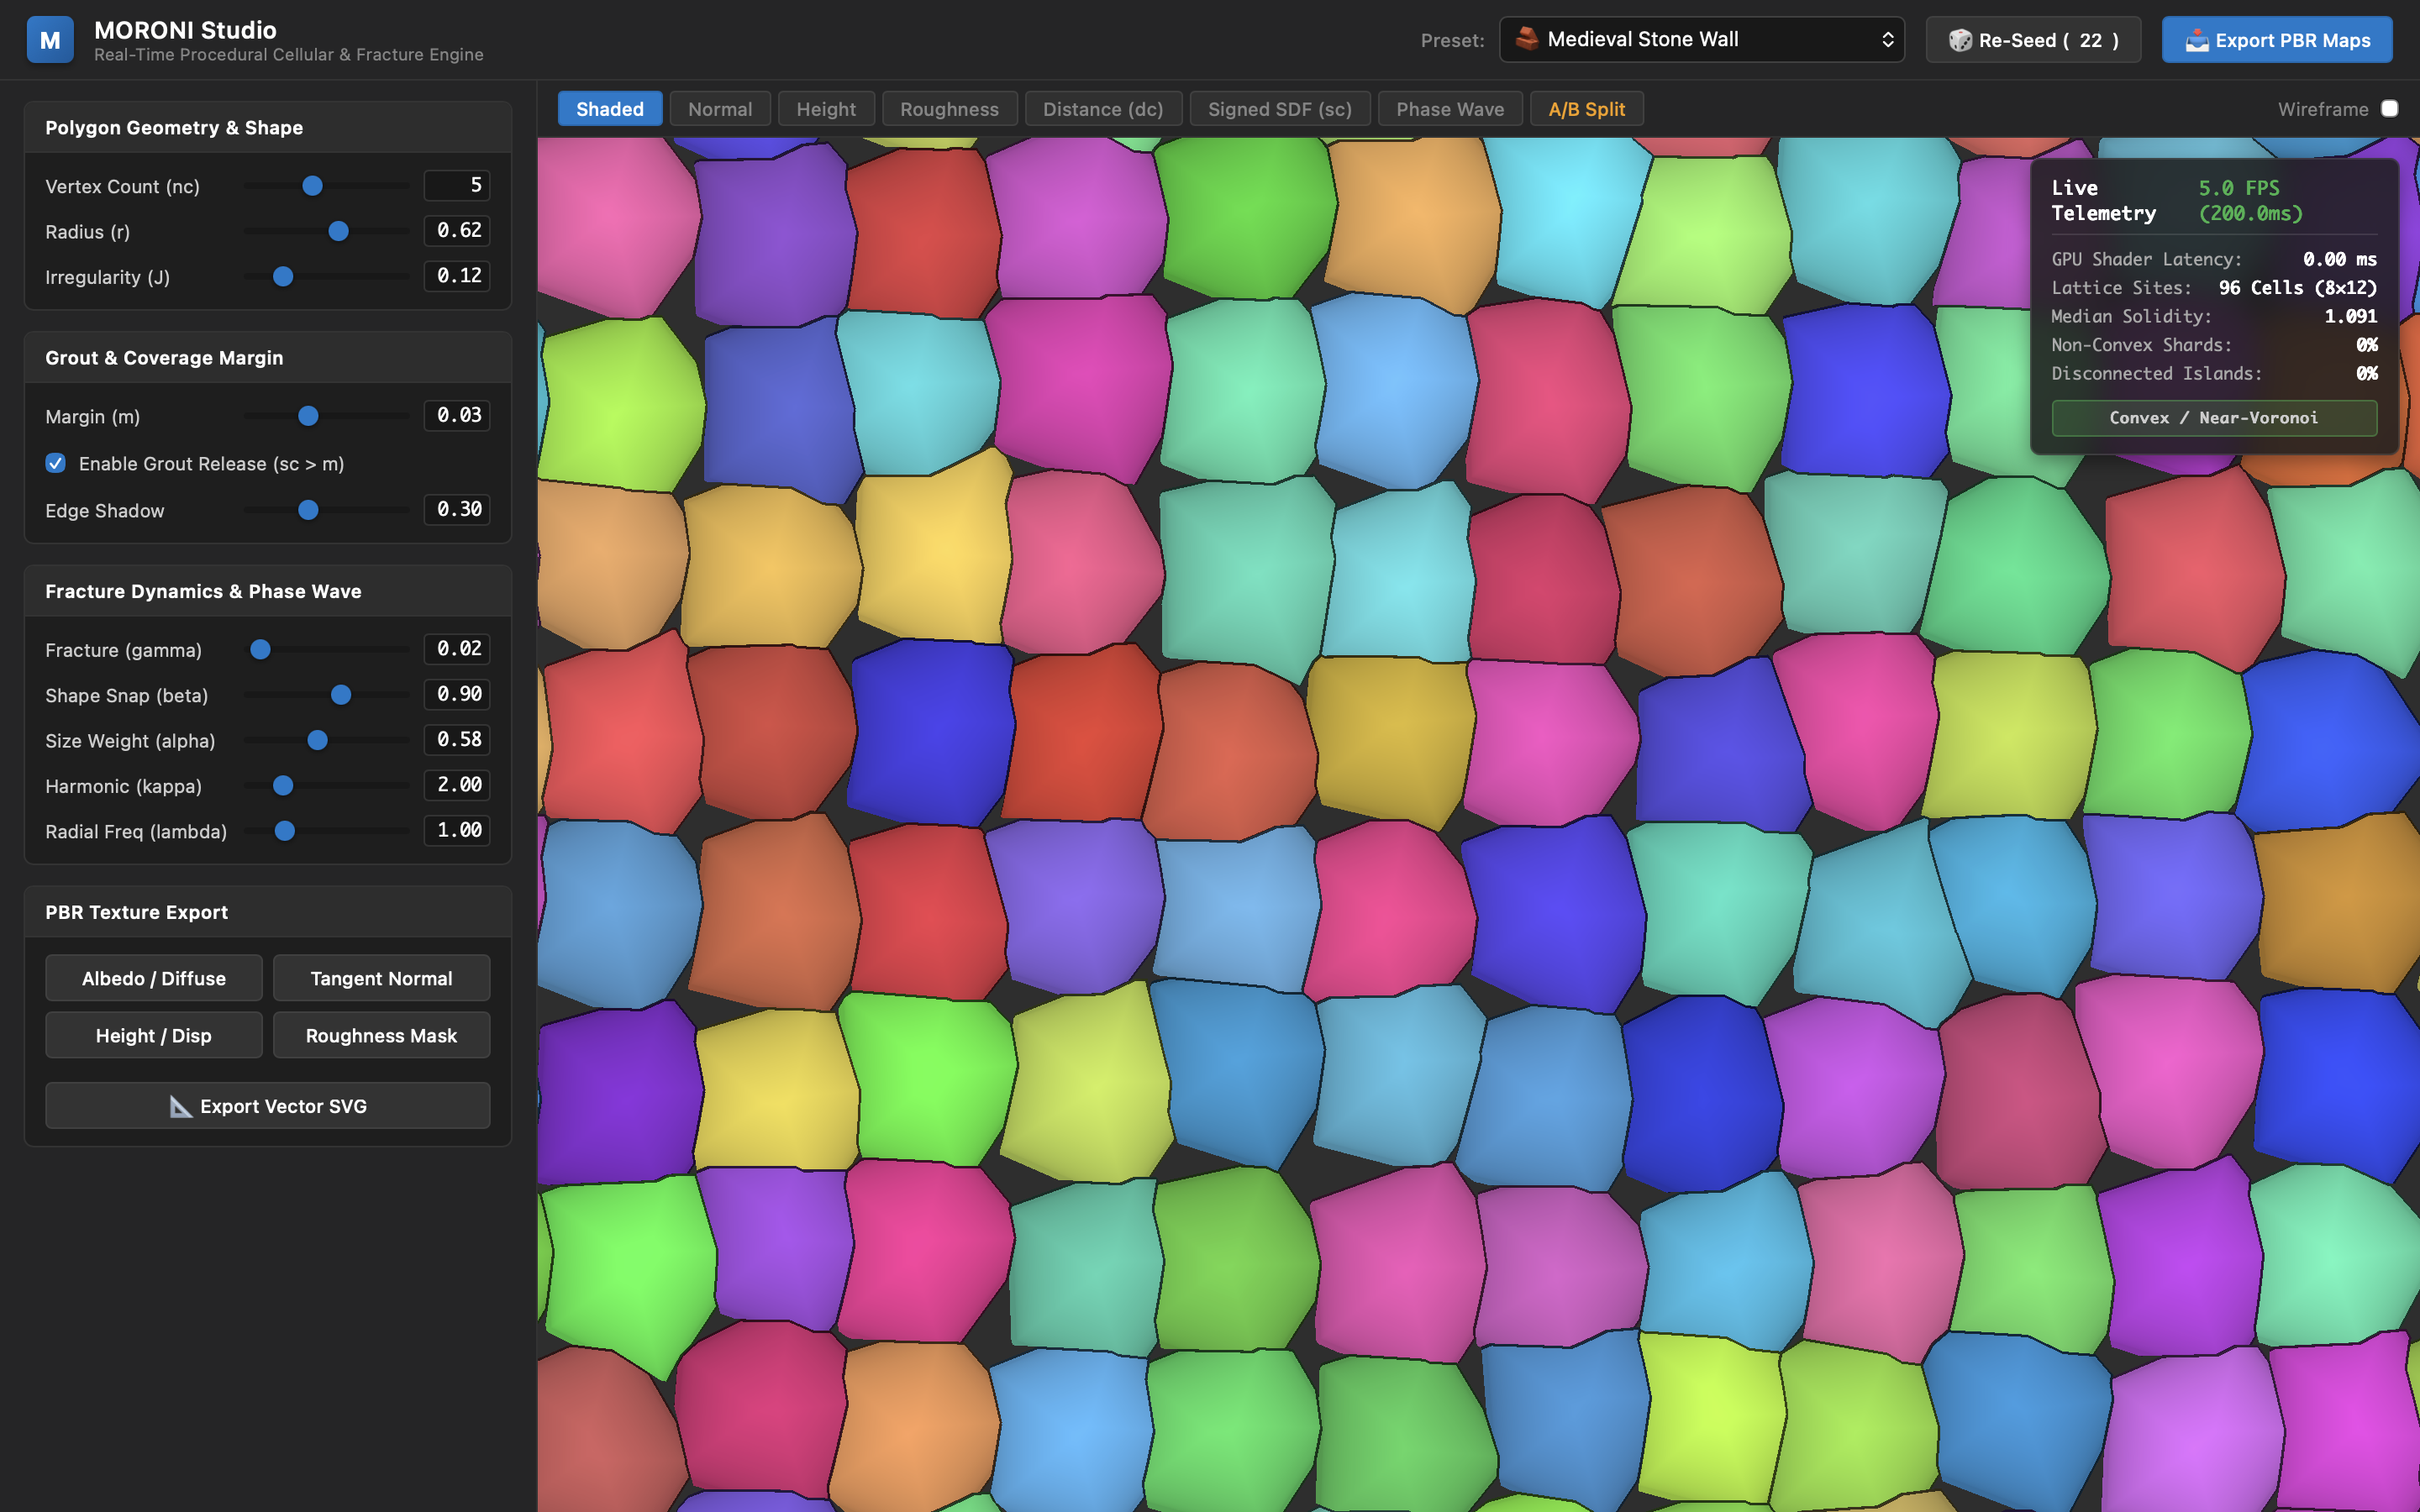
\includegraphics[width=0.85\textwidth]{figures/app_screenshot.png}
\caption{The MORONI Studio interactive laboratory interface running via WebGL2.
Left: Interactive control sidebar exposing the five art-direction dials (cell
shape $n_c$, size $r$, irregularity $J$, coverage margin $m$, and fracture
parameters $\gamma, \kappa, \lambda$), seed randomization, and PBR export
controls. Centre/Right: Interactive real-time viewport with top view-mode selector
and bottom live HUD reporting geometric solidity, non-convexity percentage,
disconnected shards, and diagram family classification.}
\label{fig:app_screenshot}
\end{figure*}

\begin{table*}[t]
\centering\scriptsize
\setlength{\tabcolsep}{2.0pt}
\caption{Comprehensive parameter specifications for the 12 production material presets available in MORONI Studio.}
\label{tbl:presets_spec}
\begin{tabular}{lcccccccccl}
\toprule
Preset Name & $n_c$ & Radius $r$ & Jitter $J$ & Margin $m$ & Use Margin & $\alpha$ & $\beta$ & $\gamma$ & $\kappa$ & Visual Surface Characteristics\\
\midrule
Stone Wall & $5$ & $0.62$ & $0.12$ & $0.03$ & \checkmark & $0.58$ & $0.90$ & $0.02$ & $2.0$ & Rectilinear masonry blocks with deep mortar recesses\\
Cracked Mud & $7$ & $0.60$ & $0.40$ & $0.05$ & \checkmark & $0.58$ & $0.32$ & $0.30$ & $2.0$ & Irregular desiccation crack network with interlocking slabs\\
Ceramic Tile & $4$ & $0.60$ & $0.02$ & $0.01$ & \checkmark & $0.58$ & $1.20$ & $0.00$ & $2.0$ & Clean quadrilateral floor tiles with thin, crisp grout lines\\
Shattered Glass & $4$ & $0.70$ & $0.50$ & $0.08$ & \checkmark & $0.58$ & $0.32$ & $0.35$ & $3.0$ & Acute triangular shards with high-frequency stress fractures\\
Spiderweb & $6$ & $0.65$ & $0.30$ & $0.04$ & \checkmark & $0.50$ & $0.35$ & $0.42$ & $4.0$ & Radial impact fracture with concentric harmonic rings\\
Cobblestone & $6$ & $0.64$ & $0.25$ & $0.06$ & \checkmark & $0.55$ & $0.75$ & $0.05$ & $2.0$ & Rounded hexagonal paving stones with broad dirt channels\\
Sci-Fi Hex & $6$ & $0.60$ & $0.00$ & $0.02$ & \checkmark & $0.58$ & $1.35$ & $0.00$ & $2.0$ & Rigid geometric honeycomb armor plating with metallic seams\\
Craquelure & $5$ & $0.55$ & $0.35$ & $0.015$ & \checkmark & $0.60$ & $0.40$ & $0.22$ & $2.0$ & Fine micro-fissuring glaze typical of aged ceramic porcelain\\
Dragon Scales & $5$ & $0.68$ & $0.18$ & $0.02$ & \checkmark & $0.52$ & $0.85$ & $0.08$ & $1.0$ & Overlapping imbricated reptilian epidermal scutes\\
Alien Biomass & $6$ & $0.62$ & $0.45$ & $0.04$ & \checkmark & $0.48$ & $0.45$ & $0.28$ & $3.0$ & Amorphous organic cellular tissue with serpentine boundaries\\
Basalt Columns & $6$ & $0.60$ & $0.08$ & $0.012$ & \checkmark & $0.58$ & $1.10$ & $0.00$ & $2.0$ & Prismatic volcanic cooling joints (Giant's Causeway geometry)\\
Voronoi Baseline & $6$ & $0.55$ & $0.00$ & $0.00$ & $\times$ & $1.00$ & $0.00$ & $0.00$ & $2.0$ & Standard nearest-site Euclidean perpendicular bisectors\\
\bottomrule
\end{tabular}
\end{table*}

\begin{figure*}[b]
\centering
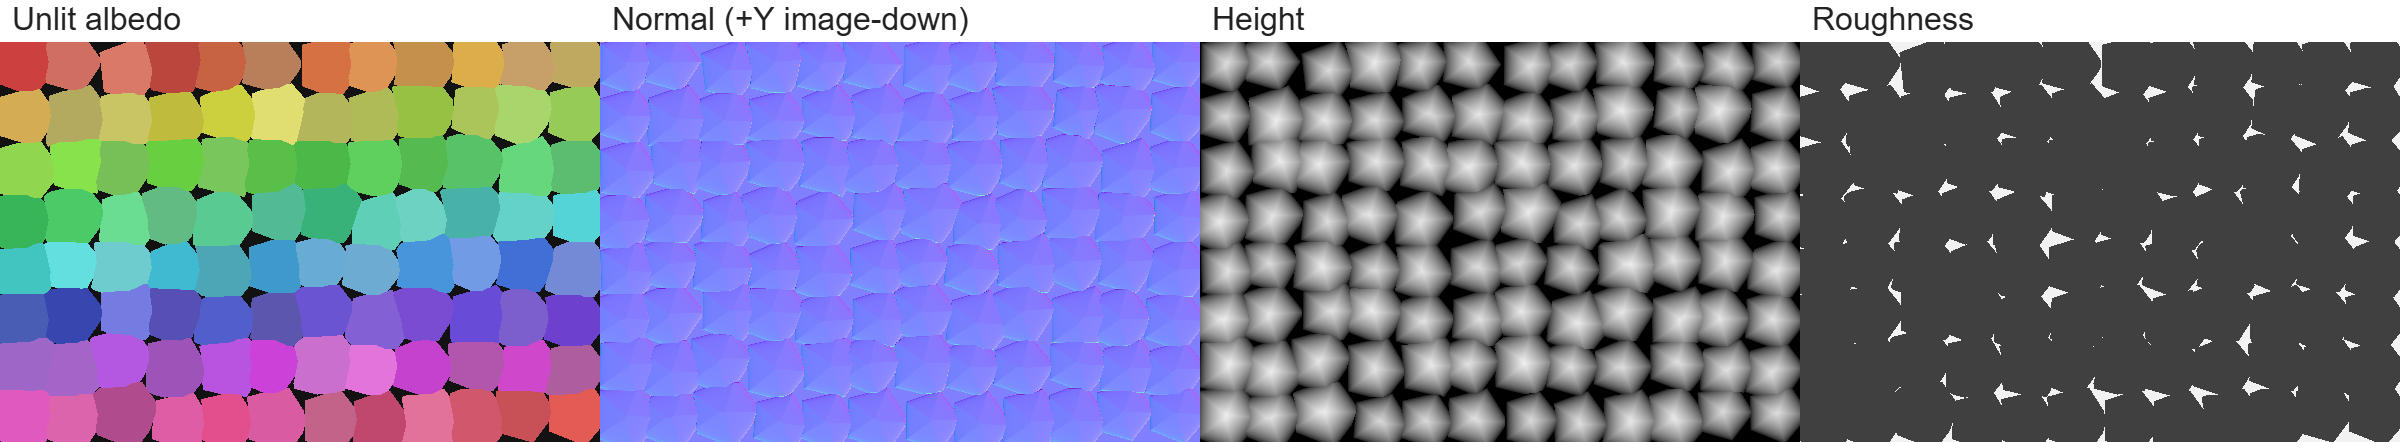
\includegraphics[width=0.65\textwidth]{figures/pbr_showcase.png}
\caption{Four-channel PBR texture maps synthesized and exported directly from the
MORONI Studio laboratory: (a) Diffuse / albedo map with darkened cell seams,
(b) Tangent-space normal map derived via central differences on the interior SDF,
(c) Height displacement map with dome curvature, and (d) Roughness / grout mask.}
\label{fig:pbr_showcase}
\end{figure*}

\subsection{Laboratory Architecture and Live Modes}

The laboratory operates entirely client-side with zero dependencies or server
requirements:
\begin{enumerate}
\item \textbf{Interactive Dials Sidebar}: Sliders provide immediate real-time
parameter binding directly to WebGL uniform buffers, updating the canvas in
sub-millisecond time.
\item \textbf{Top Viewport Mode Bar}: Allows instantaneous toggling between:
  \begin{itemize}
  \item \textbf{Shaded Texture}: Full cellular visualization with ambient cell
  shading and boundary darkening.
  \item \textbf{Tangent-Space Normal Map}: Dynamic 3D surface normals computed
  via central finite differences.
  \item \textbf{Height / Displacement Map}: Grayscale elevation map mapping
  interior signed distance to dome curvature.
  \item \textbf{Roughness / Grout Mask}: Binary/smooth mask distinguishing
  smooth cell tiles from rough recessed mortar.
  \item \textbf{Energy Field Decomposition}: Direct visual inspection of the
  isolated components: centre distance $d_c$, signed polygon field $s_c(\mathbf{x})$,
  and angular phase interference wave $(1-\cos)$.
  \item \textbf{A/B Split-Screen Comparison}: Allows dragging an interactive
  divider directly across the screen to contrast standard Voronoi against MORONI.
  \end{itemize}
\item \textbf{Live Geometric \& Topological HUD}: A real-time telemetry display
continuously tracking median cell solidity, percentage of non-convex cells, and
disconnected shard count. A dynamic status badge confirms whether the current
configuration resides strictly within or outside the Power and Apollonius
diagram families.
\end{enumerate}

\subsection{Material Preset Specifications}

Table~\ref{tbl:presets_spec} lists the parameter configurations for the 12
production material presets packaged within the studio. Figure~\ref{fig:pbr_showcase}
demonstrates the 4-channel PBR texture map export pipeline (diffuse, normal, height,
roughness), illustrating how MORONI Studio integrates into modern deferred and
physically based rendering pipelines.

\end{document}
